\documentclass[a4paper,oneside,12 pt]{article}
\usepackage[french]{babel}
\usepackage[T1]{fontenc}
\usepackage{verbatim}
\usepackage[utf8]{inputenc}
\usepackage{multirow}
\usepackage{graphicx}
\usepackage{algorithm2e}

\title{Autour de Metaciv}
\author {Gautier Maillé, Thérèse Libourel, Jacques Ferber, Julien Nigon}
\date{}
\begin{document}

\maketitle

\newpage

\tableofcontents %\clearpage$

\newpage

\part{Généralités}
\section{Introduction}
MetaCiv est un framework de développement de simulations d'évolution de sociétés humaines. Il se distingue des plateformes de simulation multi-agent générales telles que Repast, NetLogo, Gama et TurtleKit, en proposant un ensemble de constructions eco-socio-cognitives génériques permettant de gérer des agents vivant socialement dans un environnement physique en évolution.

Les principes structurels ayant guidé la conception de MetaCiv sont les suivants :

\begin{enumerate}
  \item Intégrer les aspects réactifs et cognitifs des simulations multi-agents, en disposant d’une architecture générique d’agents à base de \emph{cognitons} \cite{jacques1995systemes}.. Elle se distingue des architectures hybrides en ce sens qu’elle ne différencie pas un niveau réactif et un niveau cognitif mais qu’elle fusionne tous les facteurs aussi bien réactifs que cognitifs permettant à un agent de prendre une décision (croyances, percepts, compétences, motivations, drives, etc.). Les décisions sont prises par un système de combinaison d’influences ou poids qui déterminent la prise de décision.
  \item Utiliser les déplacements des agents comme des points d'ancrages de dynamiques émergentes, pour favoriser l'apparition de routes, de places de marchés, de lieux de rencontre, etc. On inclut, lors de la prise de décision des déplacements, des algorithmes de type A* qui prennent en compte ces lieux et constructions. Ainsi, toute modification du paysage produit une modification des comportements pouvant donner lieu à d'autres modifications du paysage (stigmergie).
  \item Intégrer les dynamiques des objets et des espaces, lesquels ont des effets en retour sur l'état des agents et des lieux.
  \item Intégrer les aspects sociaux et culturels en utilisant une extension du modèle AGR, qui fusionne les aspects culturels des groupes (normes, croyances collectives), au niveau de la prise de décision de chaque agent. Cela permet ainsi d'avoir une vision de la culture et des normes comme une motivation qui vient influencer le comportement de l'agent, et non comme des règles à prendre en compte lors d'un raisonnement.
  \item Définir et utiliser des sous-frameworks d'interaction pour modéliser le commerce, les combats, les rencontres sociales, etc.
  \item Permettre d'implémenter facilement des \emph{design patterns} cognitivo-eco-sociaux reliant les états mentaux des agents, leurs comportement, les demandes sociales, les organisations et la dynamique de l'environnement.
\end{enumerate}


\section{Méta-Modèle}

Inspiré par le modèle des \textit{quadrants}, la plateforme Metaciv est fondé sur le  méta-modèle suivant.
\begin{figure}[!h]
\begin{center}
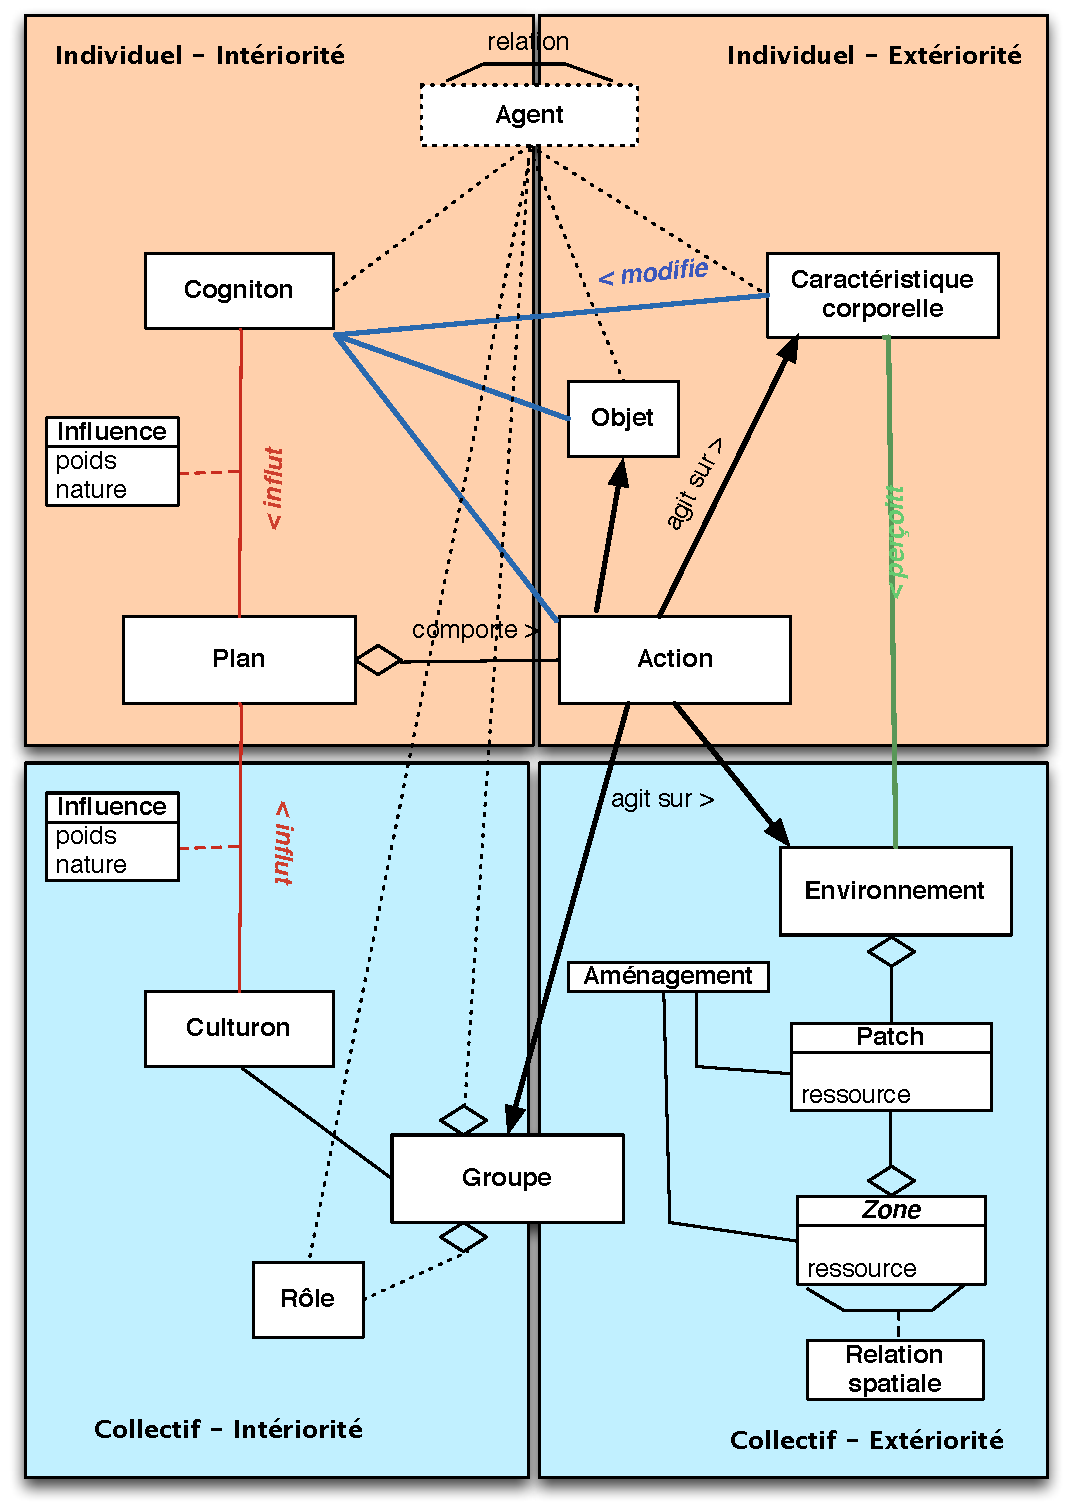
\includegraphics[scale=0.6]{modele.pdf}
\caption[Modele]{MétaModèle \\}
\label{ex1}
\end{center}
\end{figure} 
\section{Agent}
Les agents sont vus sous l'angle de \textit{l'intériorité }comme dotés d'un esprit (ensemble de cognitons) qui leur permet d'établir des plans (ensemble d'actions) ;  vus sous l'angle \textit{extériorité} ils sont dotés d'un ensemble de caractéristiques (corps) et peuvent manipuler des objets. Ils évoluent dans un environnement collectif agrégat de \textit{patches}. Côté spatialisation, ont été rajoutés les concepts de zones agrégats de patches liées par des relations spatiales (cf. relations d'Egenhofer). Sur les patches comme sur les zones l'agent peut déposer des aménagements (\textit{facility}).
Les cognitions vont influencer les plans, de manière pondérée (selon l'importance que le modélisateur leur accorde), de manière positive (renforcement) ou négative (affaiblissement).
L'environnement ainsi que les actions effectuées peuvent affecter les caractéristiques d'un agent et de ce fait influer sur ses cognitons.
De même les actions peuvent directement ou indirectement via les objets influer sur les cognitons.
\subsection{Cognition}

\subsubsection{Notion de cognitons}

	Les agents étant amenés à devoir opérer des choix dans un large panel d'actions ceux ci doivent donc disposer de capacité de réflexion et de choix suffisamment développée.
	
	Dans cette optique, l'idée retenue consiste à pondérer les différentes actions possibles pour les agents, et  ce afin de les faire choisir en fonction de ces poids. 
	Les poids des actions sont déterminés par différents facteurs : ce que voient, pensent, croient les agents… L'ensemble de ces facteurs est regroupé sous le terme de \textit{cogniton} dans ce projet, en reprenant le néologisme proposé par J. Ferber. Le cogniton est donc une « unité de pensée » qui influe sur les choix de l'agent. 	
	
	Les cognitons peuvent se cumuler, et ne sont donc pas des « états » mentaux. En fait, c'est la somme des cognitons qui représente réellement l'état mental de l'agent.
	
\subsubsection{Catégorisation des cognitons}

	Pour mieux structurer l'organisation des cognitons, ceux-ci sont catégorisés en cinq types :\textit{ Skills, Traits, Beliefs, Percepts, Mèmes}. Cette distinction permet de séparer des comportements différents entre ces cognitons, et de les traiter au mieux par la suite.
	
	
	\textit{Remarque : la catégorisatio, pour l'instant, est juste réalisée via une caractéristique du cogniton, à partir de laquelle il est possible de moduler les actions.}
	% revoir si cela est fait
\begin{itemize}


\item 	Les\textit{ Skills} (signifiant compétences en anglais) représentent les compétences, savoir-faire et connaissances techniques ou scientifiques des agents. Comme exemples de ce type de cognitons, on peut proposer : Agriculture, Navigation, Fabrication d'outils… La plupart des skills ont la particularité d'être transmissibles d'un agent à l'autre, d'être permanents (ils ne disparaissent pas une fois acquis) et d'être des prérequis indispensables à certaines actions. 
	
	Par exemple, même si d'autres cognitons l'influencent, un agent ne peut pas fabriquer un outil s'il ne dispose pas de Fabrication d'outils. Enfin, les skills sont héréditaires. Ici, on parle de l'hérédité au sens de la transmission entre les générations, ce qui représente de manière simple l'apprentissage et la transmission des connaissances.

\item 	Les \textit{Traits} représentent les spécificités individuelles de l'agent, ses traits de caractères, ses façons d'être. Des exemples possibles de ce type de cognitons sont : Ouvert, Renfermé, Paresseux…
	
	Cette catégorie n'est pas la plus importante du point de vue de la simulation et du réalisme, mais est un outil simple pour faire varier le comportement des agents si l'on veut envisager des scénarii spécifiques (des civilisations très agressives, des agents peu travailleurs, etc…). Les traits ne sont pas transmissibles d'agents à agents, sauf de manière héréditaire occasionnellement, ce qui représente l'imitation et l'éducation.

\item 	Les \textit{Beliefs} (Croyances en anglais) représentent ce que l'agent sait ou croit savoir de son environnement et de lui même. Cette catégorie est vaste, et peut regrouper des cognitons aussi variés que : Je porte une pioche, Nous sommes en guerre avec la civilisation 3, Je possède un champ. Ces cognitons ne sont généralement pas transmissibles entre agents, et ne sont pas héréditaires.

\item 	Les \textit{Percepts} représentent ce que l'agent voit, entend ou ressent (physiquement) au moment considéré. Des exemples de percepts sont : J'ai faim, Un ennemi est proche, Je suis près de l'eau. Ce type de cogniton est constamment retiré ou ajouté, contrairement aux autres types qui sont plus stables. Les percepts ne sont pas transmissibles, ils sont propres à l'agent considéré.

\item 	Les \textit{Mèmes}, d'après le terme inventé par R.Dawkins [2].
% y a t'il une biblio ?

 Son sens varie suivant les sources. Dans notre cas, nous définissons un mème comme étant une croyance ou un comportement culturel transmissible. Ainsi, les mèmes pourraient être : Je crois que l'argent est une fin en soi, je crois en l'existence d'un dieu, je crois que la démocratie est une bonne chose. Typiquement, les opinions religieuses et politiques sont des mèmes. Par définition, les mèmes sont transmissibles, et ils sont potentiellement héréditaires.
	
Les cognitons ont un poids qui par défaut est 1 (et qui peut être modifié par une action ou  par l'effet d'un objet ou par les culturons)
\end{itemize}

\subsection{Objets}
Les objets peuvent être créés, selon les besoins, par les agents (à partir de concepts d'objets précédemment définis : parmi ces concepts on distingue les objets simples et composites). Les objets feront ensuite partie de l'inventaire d'un agent. Les objets peuvent avoir un effet sur des caractéristiques d'un agent ou sur des actions. 

\subsection{Plan et actions}
Les plans sont des ensembles d'actions et sont liés à des cognitons qui les influencent.

\subsection{Groupe et rôle}
Les agents peuvent aussi appartenir à des groupes au sein desquels ils possèdent différents rôles. Le rôle d'un agent dans un groupe lui permet d'accéder à des cognitons dits \textit{ culturons} c'est-à-dire , commun à tous les agents ayant le même rôle que lui dans ce groupe. 
\newpage
\part{Le  logiciel}
\section{Préambule}
MetaCiv, dans sa forme actuelle est un \textit{framework} permettant de mettre en place des modèles de simulation de sociétés/civilisations. Il repose sur MadKit (qui offre un mécanisme de gestion multi-agents) et TurtleKit (qui fournit en particulier l’interface et la gestion « physique » des agents).

Les principaux outils fournis par MetaCiv sont :
\begin{itemize}
\item un Système « cognitif » pour les agents
\item un outil de Gestion de l’environnement à base de ressources (Cf. phéromones de Turtle Kit)
\item des Outils de visualisation
\item des Outils d’édition graphique
\end{itemize}

\section{Installation}

Il faut disposer du langage de programmation Java (version au moins 1.7) et récupérer le dossier Metaciv qui contient le dossier \textit{Launcher} ainsi que divers modèles exemples dans le Dropbox.

Ouvrir de dossier \textit{Launcher}, double clic sur le module \textit{Metaciv+numversion.jar}


Une fenêtre s'ouvre, il faut alors rechercher et ouvrir le fichier de paramètres initiaux  \texttt{parametres.metaciv} dans le modèle choisi. (Chaque modèle a un fichier de paramétrage)



\begin{figure}[hbtp]
\begin{center}
 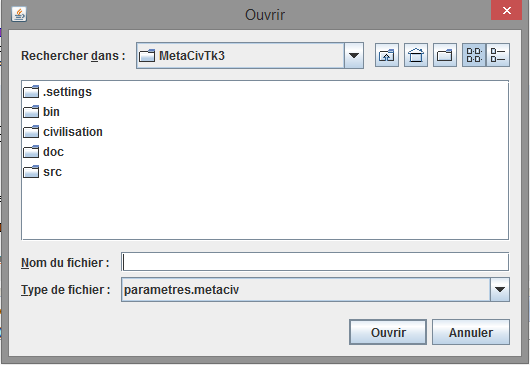
\includegraphics [scale=0.4] {ecran1.png}
\end{center}
 \caption{Le choix du fichier de paramétrage initial}
\end{figure}

%\newpage

Deux fenêtres, constituant l'environnement de fonctionnement de Metaciv  s'ouvrent alors : 
\begin{itemize}
\item l'une \textit{worldviewer} propose un fond cartographique par défaut (environnement d'évolution)

\begin{figure}[hbtp]
\begin{center}
 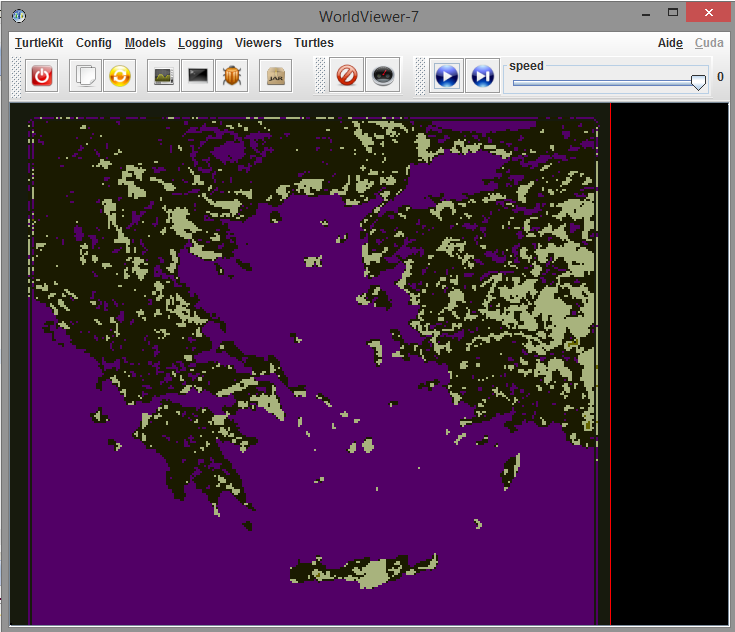
\includegraphics [scale=0.5] {worldviewer.png}
\end{center}
 \caption{La vision de l'environnement de simulation}
\end{figure}
\newpage
\item l'autre \textit{wiewertab} 

\begin{figure}[hbtp]
\begin{center}
 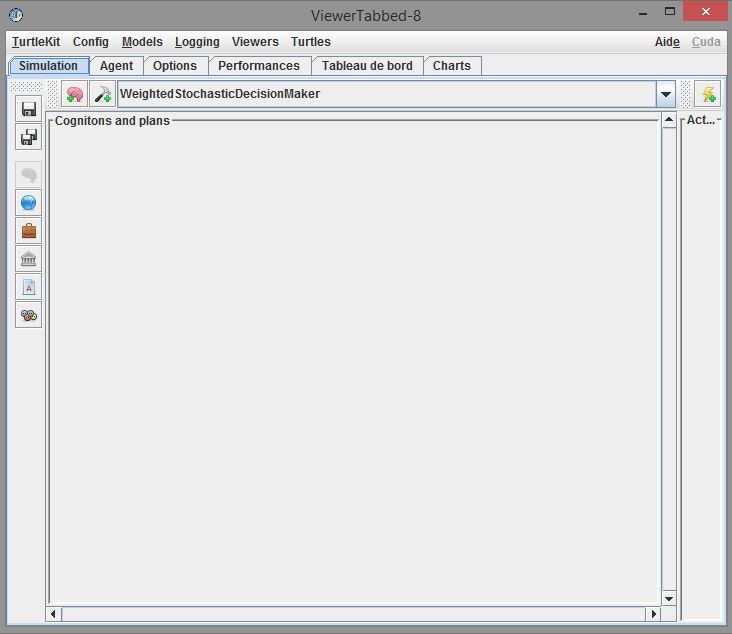
\includegraphics [scale=0.5] {viewertabbed.png}
\end{center}
 \caption{La vision de la fenêtre entrée / sortie pour le modélisateur}
\end{figure}


\end{itemize}




Les onglets de la ligne supérieure sont réservés aux experts \textit{turtlekit}.
%\newpage



La ligne suivante propose des onglets permettant d'accéder à différents détails :
\begin{figure}[hbtp]
\begin{center}
 
\includegraphics [scale=0.5] {Onglets.pdf}
\end{center}
 \caption{Les onglets accessibles }
\end{figure}


\begin{itemize}
\item L'onglet\textit{ Simulation} dispose d'une palette d'icônes permettant la création du modèle et  la modification de la simulation (cf. Figure \ref{IC}).

\begin{figure}[hbtp]
\begin{center}
 
\includegraphics [scale=0.6] {icone.pdf}
\end{center}
 \caption{Les icônes de l'onglet Simulation }
 \label{IC}
\end{figure}


%Cet onglet contient deux barres d’outils, la barre du haut varie en fonction du domaine de la simulation que l’on souhaite éditer, celle de gauche permet de naviguer grâce à des icônes parmi les différents domaines éditables.

% à voir
Le détail de ces icônes :

\begin{enumerate}
\item Les deux premières icônes : \texttt{Save} disquette permet de sauvegarder la simulation dans sa globalité, \texttt{Make copy of current save} et double disquette permet de dupliquer la dernière sauvegarde.
\item L'icône \texttt{Edit cognitive scheme}
Permet de créer et modifier cogniton et plans.
\item L'onglet \texttt{Edit Environment}
Utilisé pour  créer et modifier  les différents terrains des patches.
\item L'onglet \texttt{Edit Item}
Utilisé pour  créer et modifier les différents objets et leurs effets.
\item L'icône \texttt{Edit civilizations}
Permet de créer et modifier plusieurs populations mais constituée d'agents initialement identiques. Chaque population a un nom et un nombre d'agents.
%Par défaut il présente un ensemble d'agents homogènes ( 1 ou n) situé initialement sur un patch ou zone choisie sur l'environnement (clic droit). On peut donc au départ 

\item L'onglet \texttt{Edit Attributes}
Utilisé pour  créer et modifier pour chacune des caractéristiques (attribut) son nom et sa valeur initiale (exemple  vie 100)
\item L'onglet \texttt{Manage Groupe}
Cet onglet permet de structurer les populations initiales.
\item L'onglet \texttt{Edit Aménagement}
Cet onglet permet de créer et modifier les aménagements.
\item L'onglet \texttt{Edit Configuration}
Cet onglet permet de modifier les paramètres : nombre de messages de passages nécessaires sur un patch pour créer une route, nombre de messages de passages à enlever tous les 75 ticks (les messages sont assimilés à des phéromones et peuvent s'évaporer), nombre de patches visibles par l'agent depuis le patch où il est situé \textit{(vision)}.  % (à compléter )
\end{enumerate}




\item L'onglet \textit{Agent} : affiche des informations sur les agents, permet de sélectionner l’agent à observer.
%\item Communautés : Onglet obsolète (qui sera amené à être amélioré).
\item L'onglet \textit{Options} : permet de positionner différentes options (en particulier d’affichage). 

\item  L'onglet \textit{Performances} : présente différentes informations sur la consommation mémoire.
\item L'onglet \textit{Tableau de bord} : offre quelques outils de visualisation, par exemple le ratio des cognitons (sous forme de camembert)
\item L'onglet \textit{Charts} : présente des graphiques de synthèse et le poids des plans 

\end{itemize}

\vspace{10mm}

\textbf{Le modélisateur doit donc créer toutes entités nécessaires à son modèle (ce qui nécessite une phase de réflexion et la connaissance d'un méta-langage afin d'invoquer des codes préexistants).}


Lorsque l'univers est créé, revenir sur la fenêtre \textit{worldviewer} et cliquer sur l'icône Play (on peut régler la vitesse d'exécution) et éventuellement passer en mode pas à pas.
Il est possible d'effectuer des Zooms sur l'environnement  avec la souris 
A noter la présence du bouton fin qui clôt la simulation (impératif) et quitter le \textit{CivLauncher}.

\newpage
\part{Documentation des actions}
	
\section{Les plans}

Les plans sont des successions d'actions.
Nous distinguons trois formes de plans :
\begin{itemize}
\item  l'\textit{autoplan} qui s'exécute en toile de fond à chaque tick ; il sert à décrire des plans relatifs à la physiologie de l'agent. Il a un label bleu dans l'interface.
\item le\textit{ birthplan} s'exécute à la création de l'agent (soit à l'initialisation des peuplements, soit après la création par un agent ultérieurement). Il a un label rouge dans l'interface.

\textit{Remarque : autoplan et birthplan ne sont pas liés à des cognitons}
\item les \textit{plans} proprement dits, influencés et conditionnés par les cognitons. Un plan doit obligatoirement être conditionné par un ou plusieurs cognitons (qui doivent être dans l'esprit de l'agent pour pouvoir s'exécuter), il peut aussi être influencés par d'autres cognitons (l'influence ne s'exercera que si le cogniton origine de celle-ci est dans l'esprit de l'agent). Ils ont un label noir dans l'interface.
\end{itemize}


	
	Les actions sont exécutées à chaque pas de temps (\textit{tick}) et sur le \textit{patch} où se situe l'agent au moment de leur exécution.
	
	\textit{Remarque : il existe cependant une action logique L\_Instant qui permet d'exécuter plusieurs actions en un seul tick.}
	
	Les actions se spécialisent en actions proprement dites (préfixe A) ainsi qu'en actions logiques (préfixe L) qui regroupent des actions et d'autres actions logiques (cf. Figure \ref{HA}).
	
	\begin{figure}[!h]
	\begin{center}
	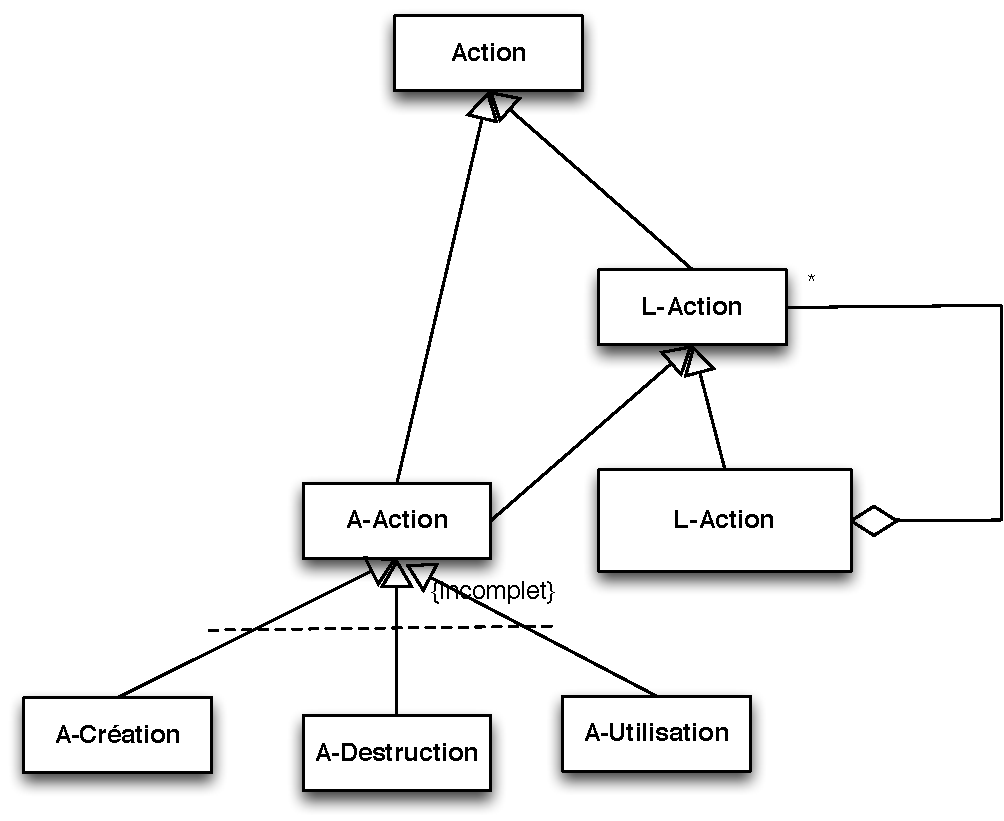
\includegraphics[scale=0.5]{DocumentationActions/HA.pdf}
	\caption[HA]{Hiérarchie des actions \\}
	\label{HA}
	\end{center}
	\end{figure}
\newpage
\section{Les actions A}
	\subsection{Les actions relatives aux objets}
	\subsubsection{A\_CreateObject} 

% modification complète de Changed Object en Modified Object

Cette action crée un objet conformément au processus de fabrication (recette ou \textit{recipe}) défini au préalable. 

La signature de l'action  est A\_CreateObject(Created Object) :
	\begin{itemize}
	\item \texttt{Created Object}, est l'objet à fabriquer.
	\end{itemize}
	
Exemple (pour un agent agriculteur) A\_CreateObject(Houe) lance la recette de fabrication de la Houe qui nécessite un bâton pour le manche et un soc (pièce métallique).
	%Cette action permet a l'agent de fabriquer un objet a partir d'autres objets présents dans son inventaire. 
	Si l'agent ne possède pas les deux objets requis pour fabriquer la houe l'action ne fera rien, sinon, elle fabriquera 1 unité de cet objet et l'ajoutera à l'inventaire de l'agent exécutant l'action. Les objets élémentaires ayant servi à la fabrication seront supprimés de l'inventaire.

\subsubsection{A\_AddObject}
Action permettant d'ajouter N objets à l'inventaire de l'agent.  

La signature de l'action est A\_AddObject(Modified Object, N) :
	\begin{itemize}
	\item \texttt{Modified Object}, précise le type d'objet utilisé pour créer directement l'objet à ajouter à l'inventaire de l'agent (sans utiliser la recette)
	\item \texttt{N}, le nombre d'objets à ajouter.
	\end{itemize}
	
	
\subsubsection{A\_DropObject}  
Action permettant de supprimer N objets de l'inventaire de l'agent.  

La signature de l'action est A\_DropItem(Modified Object, N) :	
	
	\begin{itemize}
	\item \texttt{Modified Object}, type de l'objet à retirer de l'inventaire de l'agent,
	\item \texttt{N}, le nombre d'objets à retirer.
	\end{itemize}
	
\subsubsection{A\_Transform} 

Cette action transforme une ressource prélévée sur un patch en objet.

La signature de l'action est A\_Transform (Resource to Collect, Modified Object) :
%\textit{Remarque : la ressource est appelée phéromone (hérité de Turtle Kit)}

	
	\begin{itemize}
	\item \texttt{Resource to Collect}, le type de la ressource que l'agent prélève,
	\item \texttt{Changed Object}, l'objet correspondant (pour le modélisateur) à ajouter à l'inventaire de l'agent.
	\end{itemize}
	
Exemple : un agent exécute 	 A\_Transform (Blé, Meule).

\subsubsection{A\_UseObject}
Cette action correspond à l'usage d'un objet. 


La signature de l'action est A\_UseObject(Modified Object, N) :
	\begin{itemize}
	\item \texttt{Modified Object}, le type d'objet à utiliser,
	\item \texttt{N}, le nombre.
	\end{itemize}
	
		
\subsubsection{A\_AddObjectXCogniton}

La signature de l'action est A\_AddObjectXCogniton(Modified Object, variation,base, Cogniton) :
\begin{itemize}
	\item \texttt{Modified object}, le type d'objet à ajouter,
	\item \texttt{variation}, la variation du nombre d'objets à ajouter,
	\item \texttt{base}, le nombre d'objets à ajouter par défaut,
	\item \texttt{Cogniton}, le cogniton référence.
	\end{itemize}
	
Cette action, suite à l'existence d'un Cogniton dans l'esprit de l'agent, ajoute  des objets à l'inventaire de l'agent en fonction de paramètres contextuel :
\begin{itemize}
\item  si le cogniton n'existe pas dans l'esprit de l'agent, l'action ajoute  \textit{base} objets à l'inventaire,
 \item si le cogniton existe dans l'esprit de l'agent, l'action ajoute \textit{base} + (\textit{variation} * poids de \textit{Cogniton}) objets à l'inventaire.
 \end{itemize}
	

Exemple  : un agent qui possède le Cogniton Artisan avec un poids de 2,  exécute l'action
A\_AddObjectXCogniton(Houe, 0.5,1, Artisan) ce qui lui permet d'ajouter 1+ 0.5*2 c'est-à-dire 2 Houes à son inventaire ; si l'agent ne possède pas le Cogniton Artisan l'exécution ajoute 1 seule Houe à son inventaire.
	
	
	
	\subsection{Les actions relatives aux aménagements}
	\subsubsection{A\_CreateFacility} 
	Cette action permet à l'agent de construit l'aménagement sur le patch où il se trouve au moment de l'exécution ; la signature de l'action est A\_CreateFacility(Facility) :

	\begin{itemize}
	\item \texttt{Facility}, le type d'aménagement à construire
	\end{itemize}
	
	
\subsubsection{A\_EraseFacility} 
Cette action permet à l'agent de détruire l'aménagement du  patch où il se trouve au moment de l'exécution, la signature de l'action est A\_EraseFacility(Facility) :

	\begin{itemize}
	\item \texttt{Facility}, le type d'aménagement à détruire
	\end{itemize}
	

\subsubsection{A\_GoToFacility} 
Cette action permet à l'agent d'atteindre le patch le plus proche disposant de l'aménagement (si celui ci existe) , la signature de l'action est A\_GoToAmenagement(Facility) :
	\begin{itemize}
	\item \texttt{Facility}, le type d'aménagement à cibler
	\end{itemize}
	
	.
	
\subsubsection{A\_UseFacility} 
Cette action permet à l'agent l'usage de l'aménagement (à condition qu'il soit sur le patch sur lequel se trouve l'agent), la signature de l'action est A\_UseAmenagement(Facility) :
	\begin{itemize}
	\item \texttt{Facility}, le type d'aménagement à utiliser
	\end{itemize}
	
\subsubsection{A\_DepositObjectInAmenagementLargeQuantity}

L'action permet de déposer N objets 	dans un aménagement d'un agent du groupe si l'on se trouve sur l'aménagement en question. 
La signature de l'action est A\_DepositObjectInAmenagementLargeQuantity(Modified Object, N) :
\begin{itemize}
\item Modified Object, type de l'objet à déposer dans l'aménagement.
\item N, le nombre d'objets à déposer.
\end{itemize}

\subsubsection{A\_withdrawObjectInAmenagementLargeQuantity}

L'action permet de retirer N objets dans un aménagement d'un agent du groupe si l'on se trouve sur l'aménagement en question. 
La signature de l'action est A\_withdrawObjectInAmenagementLargeQuantity(Modified Object, N) :
\begin{itemize}
\item Modified Object, type de l'objet à retirer de l'aménagement.
\item N, le nombre d'objets à retirer.
\end{itemize}

\subsubsection{A\_withdrawObjectInAmenagementHereLargeQuantity}

L'action permet de retirer N objets dans un aménagement d'un agent si l'on se trouve sur l'aménagement en question. 
La signature de l'action est A\_withdrawObjectInAmenagementHereLargeQuantity(Modified Object, N) :
\begin{itemize}
\item Modified Object, type de l'objet à retirer de l'aménagement.
\item N, le nombre d'objets à retirer.
\end{itemize}

	
	\subsection{Les actions relatives aux cognitons}
	\input{DocumentationActions/ActionsCognitons}
	
	\subsection{Les actions relatives aux déplacements}
		\subsubsection{A\_MoveTowards}  
	
	L'action permet à l'agent de se déplacer vers une cible spécifiée.
	
	\textit{Remarque : la cible aura été définie par l'action A\_GetAnotherSettlementPatch.}
	 	
 	
 	\subsubsection{A\_MoveRandomly} 
	
	L' action permet à l'agent d'effectuer un pas  dans une direction aléatoire.

\textit{Remarque : la longueur du pas dépend de la facilité de traversée du patch (cf. passability)}

	\subsubsection{A\_DoNothing}
	
	Cette action permet à l'agent de n'exécuter aucune action.
	
	\subsubsection{A\_ CreateSettlement}   
	
	Cette action permet à l'agent de se déplacer aléatoirement jusqu'à ce qu'il trouve un ensemble de patchs (les 8 patchs voisins immédiats)  dépeuplé de manière à créer un nouveau \textit{Settlement}.
	
	%\textit{Remarque : voir la terminologie }
	
	
	
	\subsubsection{A\_GetAnotherSettlementPatch}  
	
	Cette action définie la cible utilisée dans l'action A\_MoveTowards comme étant un des \textit{Settlement} pris au hasard dans l'ensemble des \textit{Settlement} existants.
	
	\subsubsection{A\_GoBackHome}
	
	Cette action permet à l'agent de se déplacer d'un pas vers son lieu de création s'il s'agit d'un des agents des peuplements initiaux, sinon vers le lieu où se trouvait l'agent qui l'a engendré.
	
	\subsubsection{A\_Move}
	
	Cette action déplace l'agent d'un pas dans une direction donnée.
	
	 La signature de cette action est A\_Move(String) :
	
	\begin{itemize}
	\item \texttt{String}, "NORTH","SOUTH","WEST","EAST" correspond à la direction que prendra  l'agent
	\end{itemize}
	
	\subsubsection{A\_SearchForResources} 
	
	Cette action permet à l'agent de rechercher autour de lui (dans son champ de vision)  la ressource passée en paramètre,  pour cela il se dirigera vers le patch le plus proche et  possédant cette ressource en quantité maximum. S'il ne trouve pas de patch contenant cette ressource, il se déplacera aléatoirement de un pas.
	
	 La signature de cette action est A\_SearchForResources(Resource To Collect) :
	
	\begin{itemize}
	\item \texttt{Resource To Collect}, correspond à la ressource recherchée.
	\end{itemize}
	
	\subsubsection{A\_SmellAndMove}
	
	Cette action permet à l'agent de chercher dans son voisinage immédiat le patch contenant la ressource passée en paramètre en plus grande quantité et de faire un pas dans sa direction. 
	
	La signature de cette action est A\_SmellAndMove(Resource To Collect) :
	
	\begin{itemize}
	\item \texttt{Resource To Collect}, correspond à la ressource recherchée.
	\end{itemize}
	
	\subsubsection{A\_GoToGroupFaicility}

Cette action ramène l'agent à un aménagement d'un des membres de son groupe.
La signature de l'action est A\_GoToGroupFaicility(Facility) :
\begin{itemize}
\item Facility, le type d'aménagement vers lequel l'agent doit se diriger.
\end{itemize}

\subsubsection{A\_GoToAmenagementInCommunity}

L'action de se rendre a l'aménagement demandé le plus proche de la civilisation. 
La signature de l'action est A\_GoToAmenagementInCommunity(Modified Object, N) :
\begin{itemize}
\item TypeAmenagement, type de l'aménagement auquel il faut se rendre.
\end{itemize}

\subsubsection{A\_FollowRoleInGroup}

L'action permet a l'agent de suivre un agent qui possède un certain rôle dans un groupe.
La signature de l'action est A\_FollowRoleInGroup(Role) :
\begin{itemize}
\item Role, de l'agent a suivre.
\end{itemize}

	\subsection{Les actions relatives aux agents}
		\subsubsection{A\_GiveBirth} 
	
	L'action permet à l'agent qui l'exécute de créer un nouvel agent sur le patch où il se situe : cet agent sera identique à ceux du peuplement initial.
	
	\subsubsection{A\_Die}
	
	L'action permet à l'agent qui l'exécute de se supprimer.
	
	\subsubsection{A\_DieIfAttributeUnderZero}
	
	L'action supprime l'agent qui l'exécute si la valeur de l'attribut (ou caractéristique) passé en paramètre descend en dessous de zéro. La signature de cette action est A\_DieIfAttributeUnderZero(attributeToCompare) :
	
	
	\begin{itemize}
	\item \texttt{attributeToCompare}, correspond à l'attribut à vérifier
	\end{itemize}	
	
	\subsubsection{A\_ChangeAttribute} 
	
	L'action modifie une caractéristique de l'agent. 
	
	La signature de l'action est A\_ChangeAttribute(Modified attribute, n) ;
	
	\begin{itemize}
	\item \texttt{Modified attribute}, correspond à la caractéristique à modifier
	\item \texttt{n}, donne la valeur à ajouter à la caractéristique
	\end{itemize}
	
	\subsubsection{A\_Trade} 
	
	L'action A\_Trade  comporte deux actions internes, elle correspond à un échange conditionnel,  car elle suppose que si après un temps fixé (\textit{turns}) l'agent n'a pas réussi à trouver un partenaire il exécute 
la deuxième action interne sinon la première.

	La signature de l'action est A\_Trade(turns, objectToGive, nObjectToGive, objectToTake, nObjectToTake, myTag, compatibleTag) ;
	
		\begin{itemize}
	\item \texttt{turns}, correspond au nombre de ticks durant lequel l'agent attend sur son patch un autre agent pour réaliser un échange,
	\item \texttt{objectToGive}  donne l'objet que l'agent échange,
	\item\texttt{nobjectToGive} correspond au nombre n d'objets à échanger,
	\item \texttt{objectToTake}  précise l'objet reçu en échange,
	\item \texttt{nobjectToTake} correspond au nombre n d'objets reçus,
	\item \texttt{mytag}, message que l'agent passe à l'attention des autres,
	\item \texttt{compatibletag} message recherché chez le partenaire échangeur potentiel.
	\end{itemize}
	
	\subsubsection{A\_TravelTrade} 
	
	L'action A\_TravelTrade  comporte deux actions internes, elle correspond à un échange conditionnel,  car elle suppose que si après un temps fixé (\textit{turns}) l'agent n'a pas réussi à trouver un partenaire il exécute la deuxième action interne sinon la première.

	La signature de l'action est A\_TravelTrade(turns, objectToGive, nObjectToGive, objectToTake, nObjectToTake, myTag, compatibleTag) ;
	
		\begin{itemize}
	\item \texttt{turns}, correspond au nombre de ticks durant lequel l'agent cherche des partenaires commerciaux dans son voisinage et se déplace vers eux,
	\item \texttt{objectToGive}  donne l'objet que l'agent échange,
	\item\texttt{nobjectToGive} correspond au nombre n d'objets à échanger,
	\item \texttt{objectToTake}  précise l'objet reçu en échange,
	\item \texttt{nobjectToTake} correspond au nombre n d'objets reçus,
	\item \texttt{mytag}, message que l'agent passe à l'attention des autres,
	\item \texttt{compatibletag} message recherché chez le partenaire échangeur potentiel.
	\end{itemize}
	
	
	\subsubsection{A\_CreateGroup}
	
	L'action permet à l'agent  de créer un groupe. 
	
	La signature de l'action  est A\_CreateGroup(GroupToCreate) : 
	
	\begin{itemize}
	\item \texttt{GroupToCreate}, donne le type du groupe à créer.
	\end{itemize}
	
	\subsubsection{A\_HireForRole}
	
	L'action permet à l'agent exécutant d'ajouter un agent présent sur le même patch que lui à son groupe . 
	
	La signature de l'action est A\_HireForRole(GroupToCreate) :
	
	\begin{itemize}
	\item \texttt{GroupToCreate}, donne  le type du groupe dans lequel  l'agent sera admis
	\end{itemize}
	
	\textit{Remarque : un agent peut appartenir à plusieurs groupes}
	
	
	\subsubsection{A\_DisbandGoup}

Cette action détruit un groupe et retire tout les membres de celui-ci
La signature de l'action est A\_DisbandGoup(Groupe) :
\begin{itemize}
\item Groupe, le nom du groupe auquel appartient l'agent qui détruit le groupe.
\end{itemize}

\subsubsection{A\_CreatedElectedGroup}

Cette action a pour but la création d'un groupe a travers un vote. Si 50\% des votants approuve la motion, alors tout les votant rejoingne le groupe dans un certain role et le demander du vote dans un autre. 
La signature de l'action est A\_CreatedElectedGroup(Role, Role, cogniton, attribut) :
\begin{itemize}
\item Role, le nom du role dont le demandeur va rejoindre.
\item Role, le nom du role dont les votant vont rejoindre.
\item cogniton, le cogniton surlequel se base le vote.
\item attribut, le nom de l'attribut qui conditionnent le vote des votant.\end{itemize}


\subsubsection{A\_HireForRole}

Cette action recrute un agent sans groupe se trouvant sur le même patch que l'agent et lui donne un rôle dans son groupe.
La signature de l'action est A\_HireForRole(Role) :
\begin{itemize}
\item Role, le rôle dans lequel le nouvel agent recruté sera affecté dans le groupe.
\end{itemize}

\subsubsection{A\_AskRandomMemberToChangeRoleForAnother}

Cette action change le rôle d'un des membre du groupe de l'agent pour un autre rôle spécifié (s'il n'est pas déjà dans ce rôle).
La signature de l'action est A\_AskRandomMemberToChangeRoleForAnother(Role):
\begin{itemize}
\item Role, le rôle vers lequel un membre du groupe se convertira.
\end{itemize}

\subsubsection{A\_BirthGroupAndRole}

Cette action ressemble à l'action A\_Birth, elle créer un nouvel agent en appelant le BirthPlan puis ajoute le nouveau membre au groupe en lui affectant un rôle.
La signature de l'action est A\_BirthGroupAndRole(Role):
\begin{itemize}
\item Role, le rôle vers lequel le nouvel agent sera affecté dans le groupe.
\end{itemize}

\subsubsection{A\_ChangeAttributeDouble}

Cette action ressemble à l'action A\_ChangeAttribute, elle permet de modifier l'attribut d'un agent en ajoutant un N (double) à la valeur de l'attribut.
La signature de l'action est A\_ChangeAttributeDouble(Modified Attribute, N):
\begin{itemize}
\item Modified Attribute, attribut de l'agent à modifier.
\item N, la valeur à ajouter à la valeur de l'attribut.
\end{itemize}

\subsubsection{A\_ChangeRoleForAnother}

Cette action change le rôle de l'agent pour un autre rôle du groupe.
La signature de l'action est A\_ChangeRoleForAnother(Role):
\begin{itemize}
\item Role, le rôle vers lequel l'agent se convertira.
\end{itemize}

\subsubsection{A\_DieAndRemoveFacilities}

Cette action fait mourir l'agent et efface tous ses aménagements.
Cette action ne possède pas d'arguments.

\subsubsection{A\_DieAndRemoveSpecificFacility}

Cette action fait mourir l'agent et n'efface qu'un type d'aménagement.
La signature de l'action est A\_DieAndRemoveSpecificFacility(Facility):
\begin{itemize}
\item Facility, le type d'aménagements supprimés à la mort de l'agent.
\end{itemize}


\subsubsection{A\_setPoissonLaw}

Cette action modifie un attribut et lui donne la valeur d'un nombre suivant un loi de poisson de paramètre $\lambda = 10$ et $n=20$ et multiplié par 5.
La signature de l'action est A\_setPoissonLaw(Modified Attribute):
\begin{itemize}
\item Modified Attribute, est l'attribut modifié.
\end{itemize}
	
\section{Les actions L}

\subsection{Tests}


La structure générale des actions logiques de type Test est :

\begin{algorithm}
\Begin{
       
    \If{ condition }
  			 { 
  		 		action interne 1 
  		 		
   			}	   
        	\Else
        	{
        		action interne 2 
        		    	
        	}
   }  
  
\end{algorithm}

\newpage
\textit{Remarque : ces actions logiques sont toutes composées de deux actions internes (qui peuvent elles-mêmes être composites).}

Les diverses actions suivantes vont préciser le type de condition.

\subsubsection{L\_CompareAttribute}
La condition porte sur la valeur d'un attribut de l'agent.

La signature de cette action est L\_CompareAttribute(attributTocompare, comparator, n) :
\begin{itemize}
	\item \texttt{attributTocompare}, est l'attribut concerné,
	\item \texttt{comparator} l'opérateur de comparaison $<$, $>$, $<=$,$ >=$,$ ==$,
	\item \texttt{n} la valeur de comparaison.
	\end{itemize}

\subsubsection{L\_CompareObject}
La condition porte sur le nombre d'objets d'un type donné possédés.

La signature de cette action est L\_CompareObject(objectTocompare, comparator, n) :
\begin{itemize}
	\item \texttt{objectTocompare}, est le type d'objet concerné,
	\item \texttt{comparator} l'opérateur de comparaison $<$, $>$, $<=$,$ >=$,$ ==$,
	\item \texttt{n} le nombre d'objets.
	\end{itemize}
\subsubsection{L\_CompareResource}
La condition porte sur la valeur de la ressource présente sur le patch où est situé  l'agent.

La signature de cette action est L\_CompareResource(resourceTocompare, comparator, n) :
\begin{itemize}
	\item \texttt{resourceTocompare}, est le type de la ressource concernée,
	\item \texttt{comparator} l'opérateur de comparaison $<$, $>$, $<=$,$ >=$,$ ==$,
	\item \texttt{n} la valeur de la ressource.
	\end{itemize}
	
	
\subsubsection{L\_IsFacilityHere}

La condition teste la présence de l'aménagement \textit{(facility)} concerné sur le patch  où est situé  l'agent.

La signature de cette action est L\_IsFacilityHere(facility) :
\begin{itemize}
	\item \texttt{facility},  le type d'aménagement testé.
	\end{itemize}	
	
\subsubsection{L\_IsAnyFacilityHere}
La condition teste la présence d'un aménagement de n'importe quel type sur le patch  où est situé  l'agent.

\subsubsection{L\_OwnFacility}

La condition teste la possession d'un aménagement donné.

La signature de cette action est L\_OwnFacility(facility) :
\begin{itemize}
	\item \texttt{facility},  le type d'aménagement testé.
	\end{itemize}	
\subsubsection{L\_OwnCogniton}
La condition teste la possession d'un cognition.

La signature de cette action est L\_OwnCogniton(cogniton) :
\begin{itemize}
	\item \texttt{cogniton},  le type de cogniton testé.
	\end{itemize}	
\subsubsection{L\_OwnObject}

La condition teste la possession d'un objet. 

La signature de cette action est L\_OwnObject(object) :
\begin{itemize}
	\item \texttt{object},  le type d'objet testé.
	\end{itemize}	

\subsubsection{L\_IsAmenagementInCommunity}

La condition porte sur la présence d'un aménagement dans la civilisation. Il s'agit de tester si ce type d'aménagement est présent.
La signature de cette action est L\_CompareAttributeToAttribute(TypeAmenagement):
\begin{itemize}
\item TypeAmenagement est le type d'aménagement attribut concerné.
\end{itemize}


\subsubsection{L\_CompareAttributeToAttribute}

La condition porte sur les valeurs de deux attributs de l'agent, elles sont comparés par un comparateur.
La signature de cette action est L\_CompareAttributeToAttribute(Attribute1, comparator, Attribute2):
\begin{itemize}
\item Attribute1 est le premier attribut concerné.
\item comparator est l'opérateur de comparaison $<, >, \leq, \geq, == $.
\item Attribute2 est le deuxième attribut concerné.
\end{itemize}

\subsubsection{L\_CompareAttributeToConstant}

La condition porte sur la valeur d'un attribut par rapport à une constante.
La signature de cette action est L\_CompareAttributeToConstant(Attribute, comparator, Constant):
\begin{itemize}
\item Attribute est l'attribut concerné.
\item comparator est l'opérateur de comparaison $<, >, \leq, \geq, == $.
\item Constant est la constante concernée.
\end{itemize}

\subsubsection{L\_CompareGroupAttributeToPopulation}

La condition porte sur un la somme des attributs des membres d'un groupe par rapport au nombre d'individus de ce groupe.
La signature de cette action est L\_CompareGroupAttributeToPopulation(Attribute, comparator):
\begin{itemize}
\item Attribute, est l'attribut de groupe à comparer.
\item comparator est l'opérateur de comparaison $<, >, \leq, \geq, == $.
\end{itemize}

%L\_CompareNombreObjets
%L\_CompareNombreObjetsInGroupAmenagement

\subsubsection{L\_CompareRoleMembers}

La condition porte sur le nombre d'individus du groupe par rapport à un nombre N.
La signature de cette action est L\_CompareRoleMembers(N, comparator):
\begin{itemize}
\item N est le nombre à comparer à la population du groupe.
\item comparator est l'opérateur de comparaison $<, >, \leq, \geq, == $.
\end{itemize}

\subsubsection{L\_IsInThatGropInThatRole}

La condition porte sur le rôle de l'agent dans son groupe.
La signature de cette action est L\_IsInThatGropInThatRole(Role):
\begin{itemize}
\item Role, le rôle à comparer avec le rôle de l'agent.
\end{itemize}


\subsection{Algorithmiques}

Ces actions logiques composites sont associées à des structures standard algorithmique.



\subsubsection{L\_Instant}

Cette action composite effectue la globalité de ses actions internes en un seul tick.



\subsubsection{L\_Random}
Cette action composite effectue une seule de ses actions internes choisie aléatoirement en un seul tick.


\subsubsection{L\_RandomPercent}

Cette action composite n'a que deux actions internes et choisit selon le pourcentage l'action interne à exécuter.

La signature de cette action est L\_RandomPercent(n) :
\begin{itemize}
	\item \texttt{n},  le pourcentage de chance qu'à l'action interne 1 de s'exécuter.
	\end{itemize}	
	
\subsubsection{L\_Repeat}
Cette action composite ne comporte qu'une action interne qu'elle va exécuter n fois en n tick.

La signature de cette action est L\_Repeat(n) :
\begin{itemize}
	\item \texttt{n},  le nombre d'itérations.
	\end{itemize}	



	
	
	
\newpage
\part{Outils de création d'un modèle}
	\section{Phase d'initialisation}
\subsection{Peuplements}
Dans la fenêtre \textit{Wiewertabs}, cliquer sur l'icône \textit{Edit civilisation}, sur la droite la liste des peuplements existants (par défaut  rattaché à l'environnement par défaut).
Pour créer un nouveau peuplement, cliquer sur l'icône \textit{create new civilization},   donner son nom (par exemple Volque), sa population (par exemple 100) et valider (touche entrée).

\subsection{Environnement physique}

Dans la fenêtre \textit{Wiewertabs}, cliquer sur l'icône \textit{Edit environnement}, la liste des terrains attribuables aux \textit{patches} et  définis dans le dossier de la simulation apparait dans la partie droite de la fenêtre (cf. Figure \ref{ENV}).
\begin{figure}[!ht]
	\begin{center}
	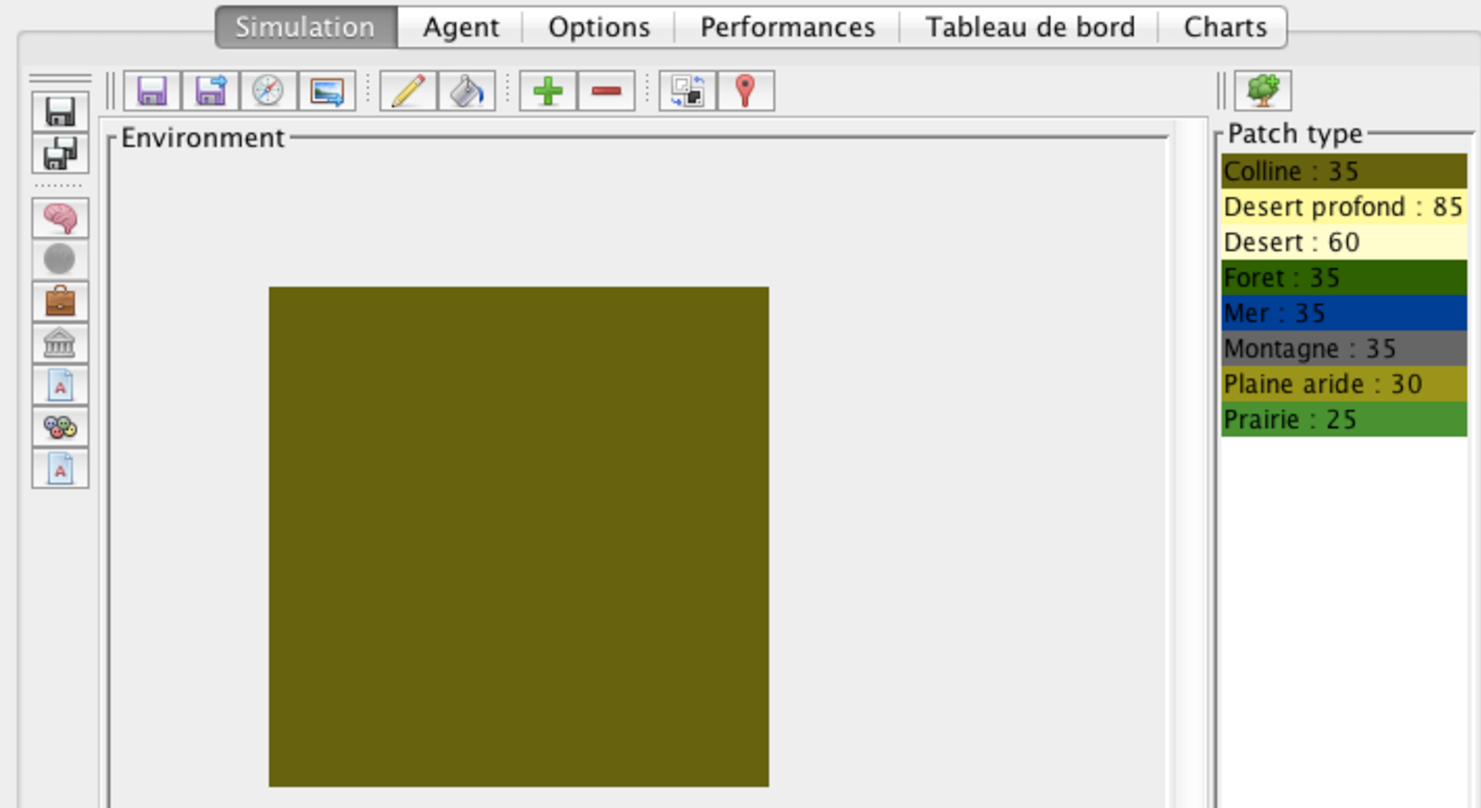
\includegraphics[scale=0.4]{DocumentationSimulation/Env.pdf}
	\caption[ENV]{Environnement \\}
	\label{ENV}
	\end{center}
	\end{figure}
	
Pour la simulation deux terrains sont utilisés \textit{Forêt} et \textit{Prairie} avec une valeur liée à leur facilité de traversée (\textit{passability}).

Les modifications sur un terrain se font par l'intermédiaire d'un clic droit sur le terrain voulu.
On peut alors éditer, changer la couleur ou supprimer le terrain.
Si on édite notre exemple (cf. Figure \ref{Ter} ), on observe le terrain \textit{Prairie} avec la valeur 25 pour \textit{passability}, puis une liste d'attributs correspondant chacun à un type de ressource disponible sur le terrain. Pour chaque ressource on peut attribuer une valeur initiale et une valeur de croissance (à chaque\textit{ tick}). 

\begin{figure}[!ht]
	\begin{center}
	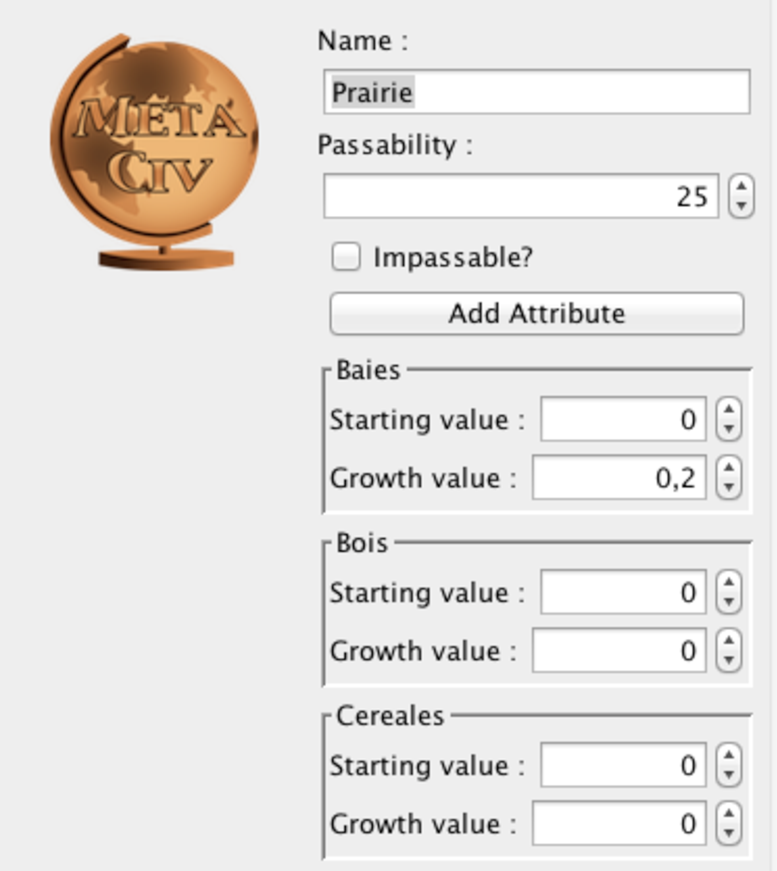
\includegraphics[scale=0.5]{DocumentationSimulation/terrain.pdf}
	\caption[Ter]{Edition d'un terrain \\}
	\label{Ter}
	\end{center}
	\end{figure}


% On peut aussi ajouter de nouveaux attributs (ressources).

Dans la partie centrale de la fenêtre, l'environnement global peut être construit, dimensions (icône boussole \textit{set environment bounds}), chargement d'un environnement existant (icône \textit{Load Environment}), définir à partir d'une image (\textit{generate an environment from an existing picture}) ou dessiner (icône crayon et pot de peinture). 

On peut sauvegarder l'environnement (icône disquette), choisir l'environnement de la simulation (qui peut donc être un autre) icône \textit{choose environment to use for simulation}, et ajouter des ressources à l'environnement (icône \textit{manage pheronom}).


Dernière chose, situer le ou les peuplements sur l'environnement : pour cela clic droit sur la position voulue (possibilité de zoom) et donner le nom du peuplement dans la fenêtre qui s'ouvre (et penser à sauvegarder).

\begin{figure}[!ht]
	\begin{center}
	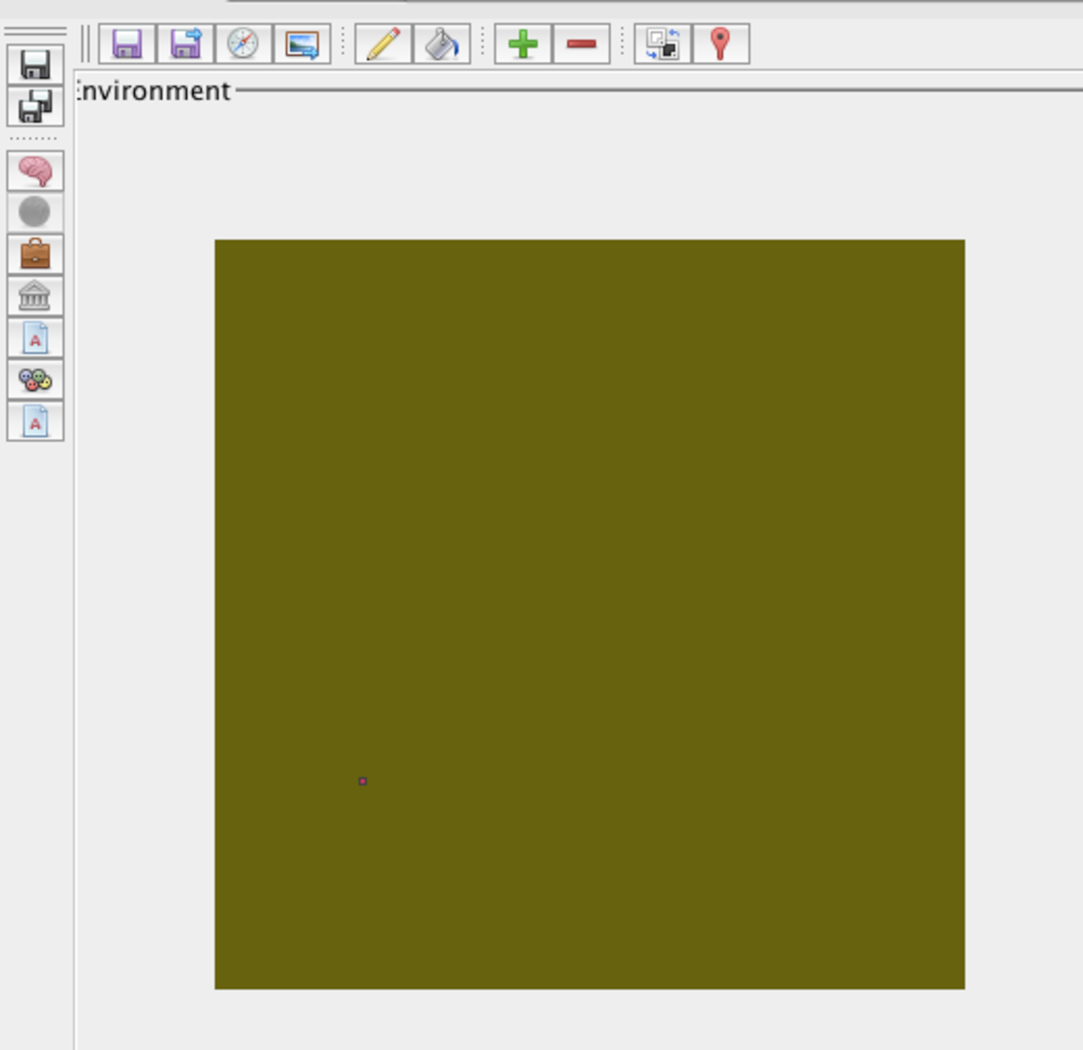
\includegraphics[scale=0.4]{DocumentationSimulation/Local.pdf}
	\caption[Lo]{Localisation du peuplement, le point marque la localisation}
	\label{Lo}
	\end{center}
	\end{figure}
	
\subsection{Les objets}
Dans la fenêtre \textit{Wiewertabs}, cliquer sur l'icône \textit{Edit Item}.

Sur la partie droite une liste d'objets apparaît et en cliquant sur l'icône \textit{Add Item} on accède à la fenêtre suivante (cf. Figure \ref{Obj}).

\begin{figure}[!ht]
	\begin{center}
	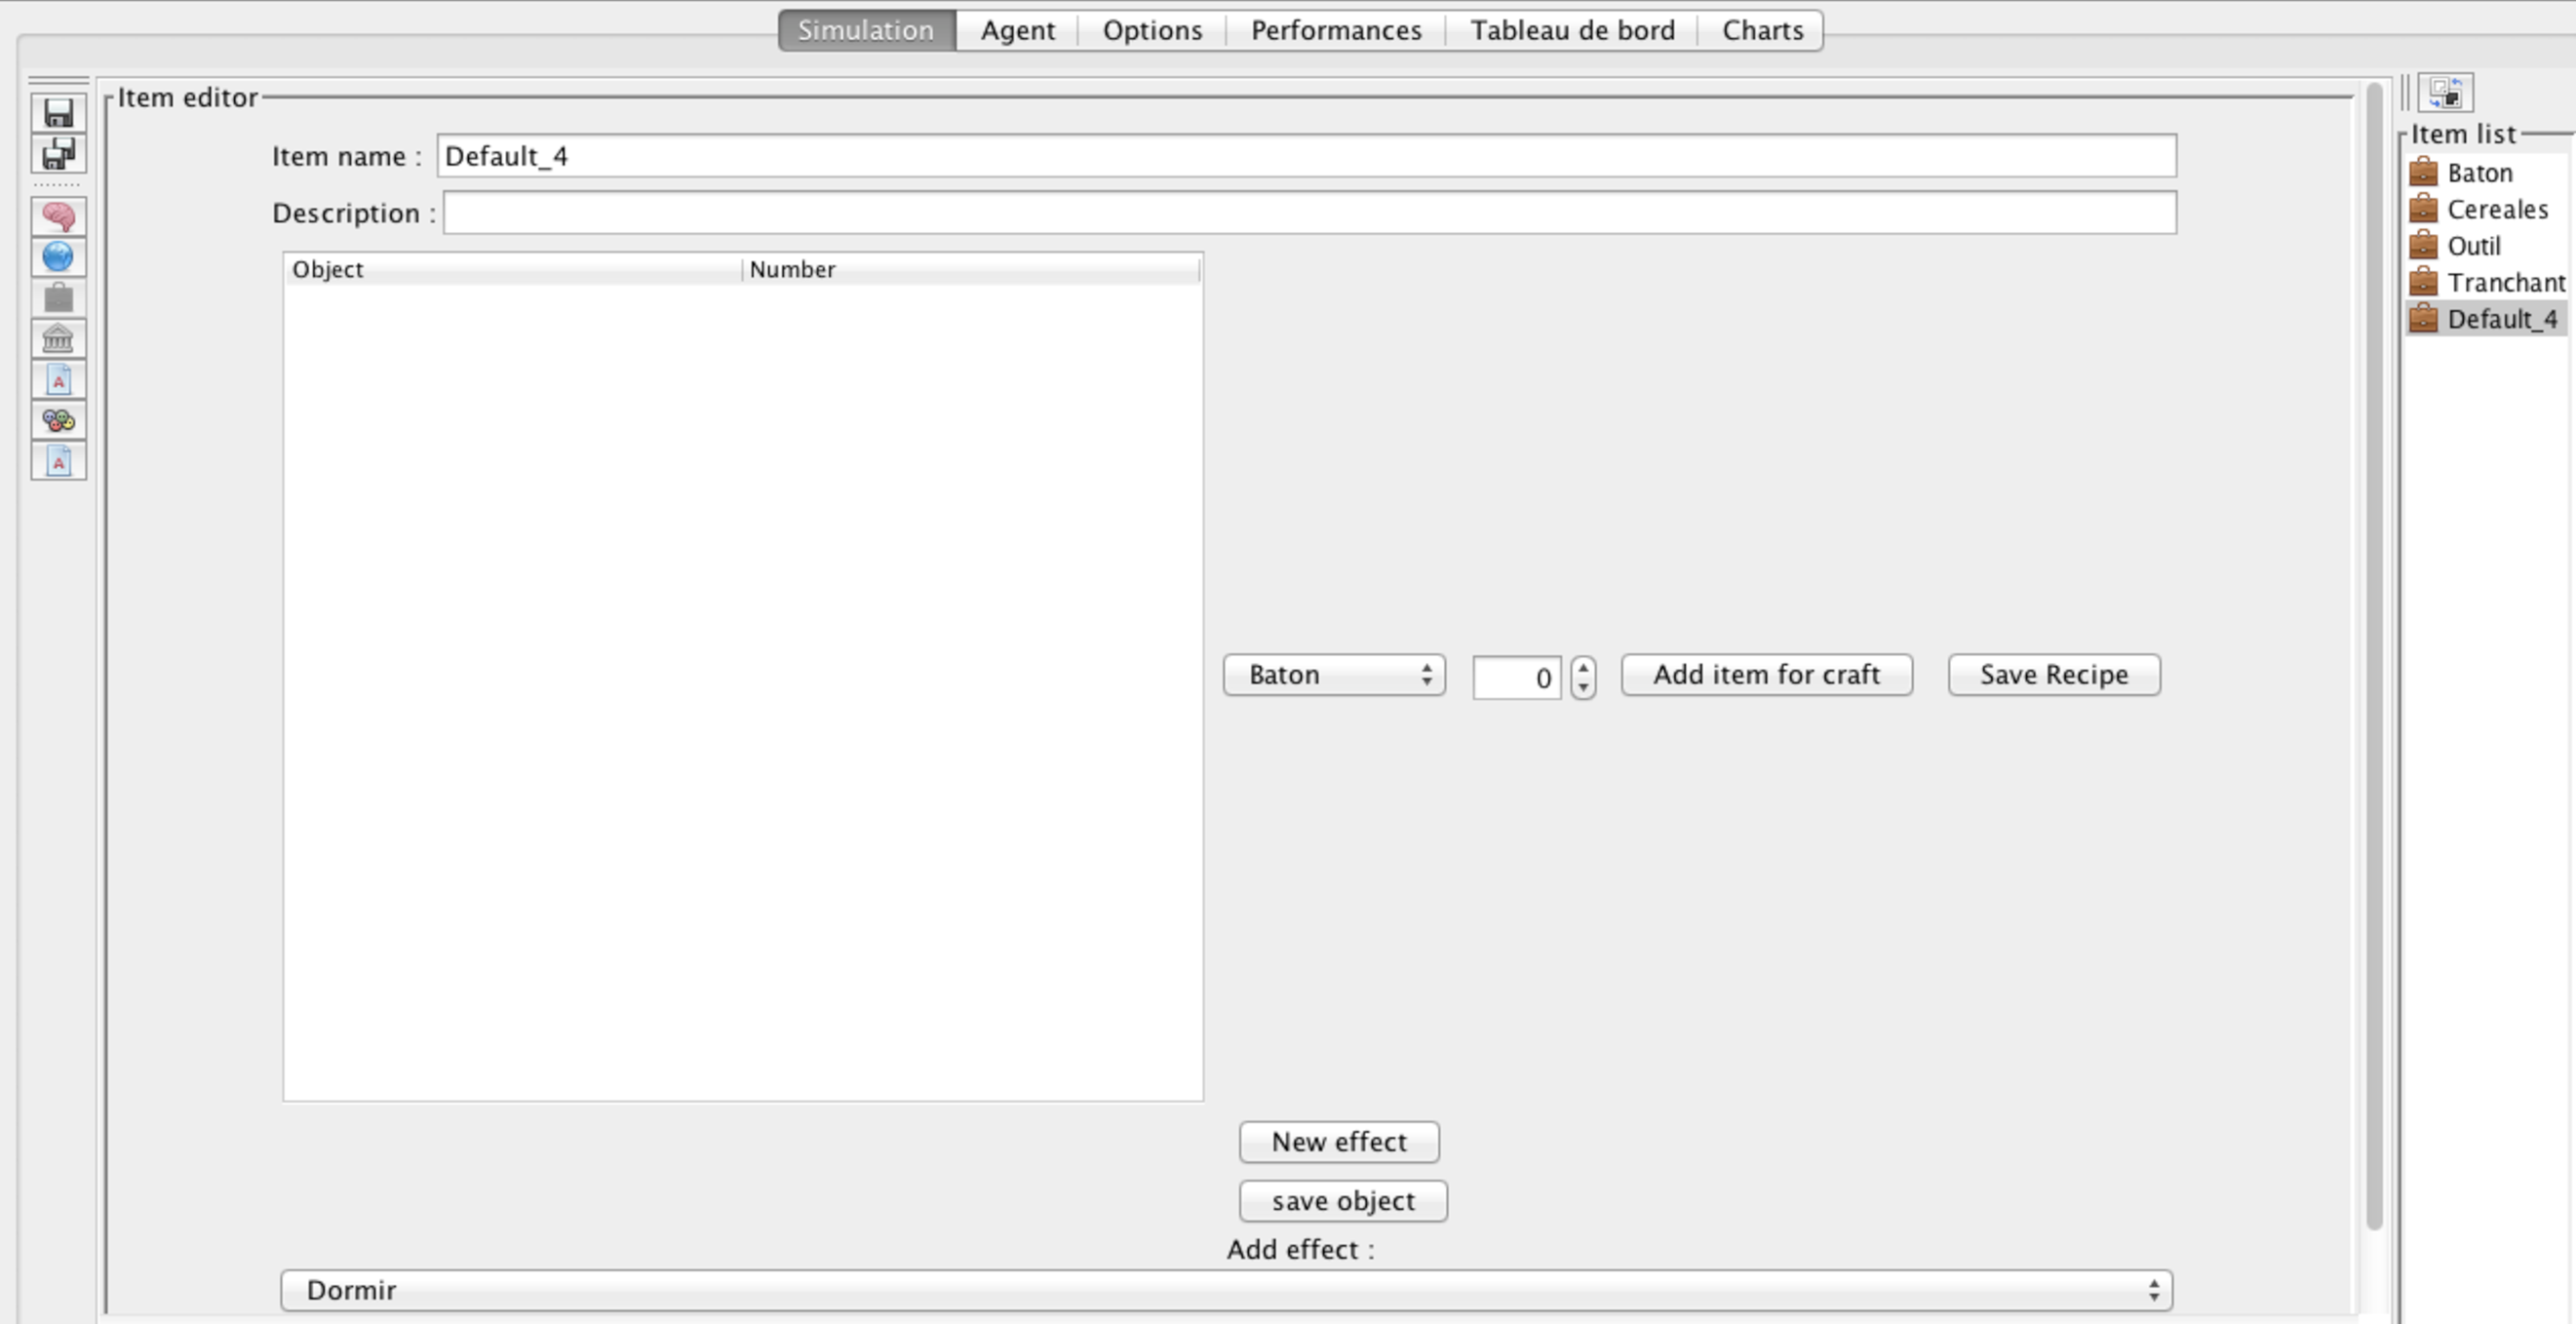
\includegraphics[scale=0.3]{DocumentationSimulation/Objet.pdf}
	\caption[Obj]{Ajout d'objet \\}
	\label{Obj}
	\end{center}
	\end{figure}
	
Dans cette fenêtre donner un nom et une description à l'objet avant de sauvegarder.

Si l'on souhaite créer des descriptions d'objet complexe, on peut saisir le nom et le nombre d'éléments constitutifs (ce qui constitue la recette ou \textit{recipe}). 

On peut de plus ajouter des effets existants ou en créer de nouveaux (cf. Figure \ref{Ob2}).
\begin{figure}[!ht]
	\begin{center}
	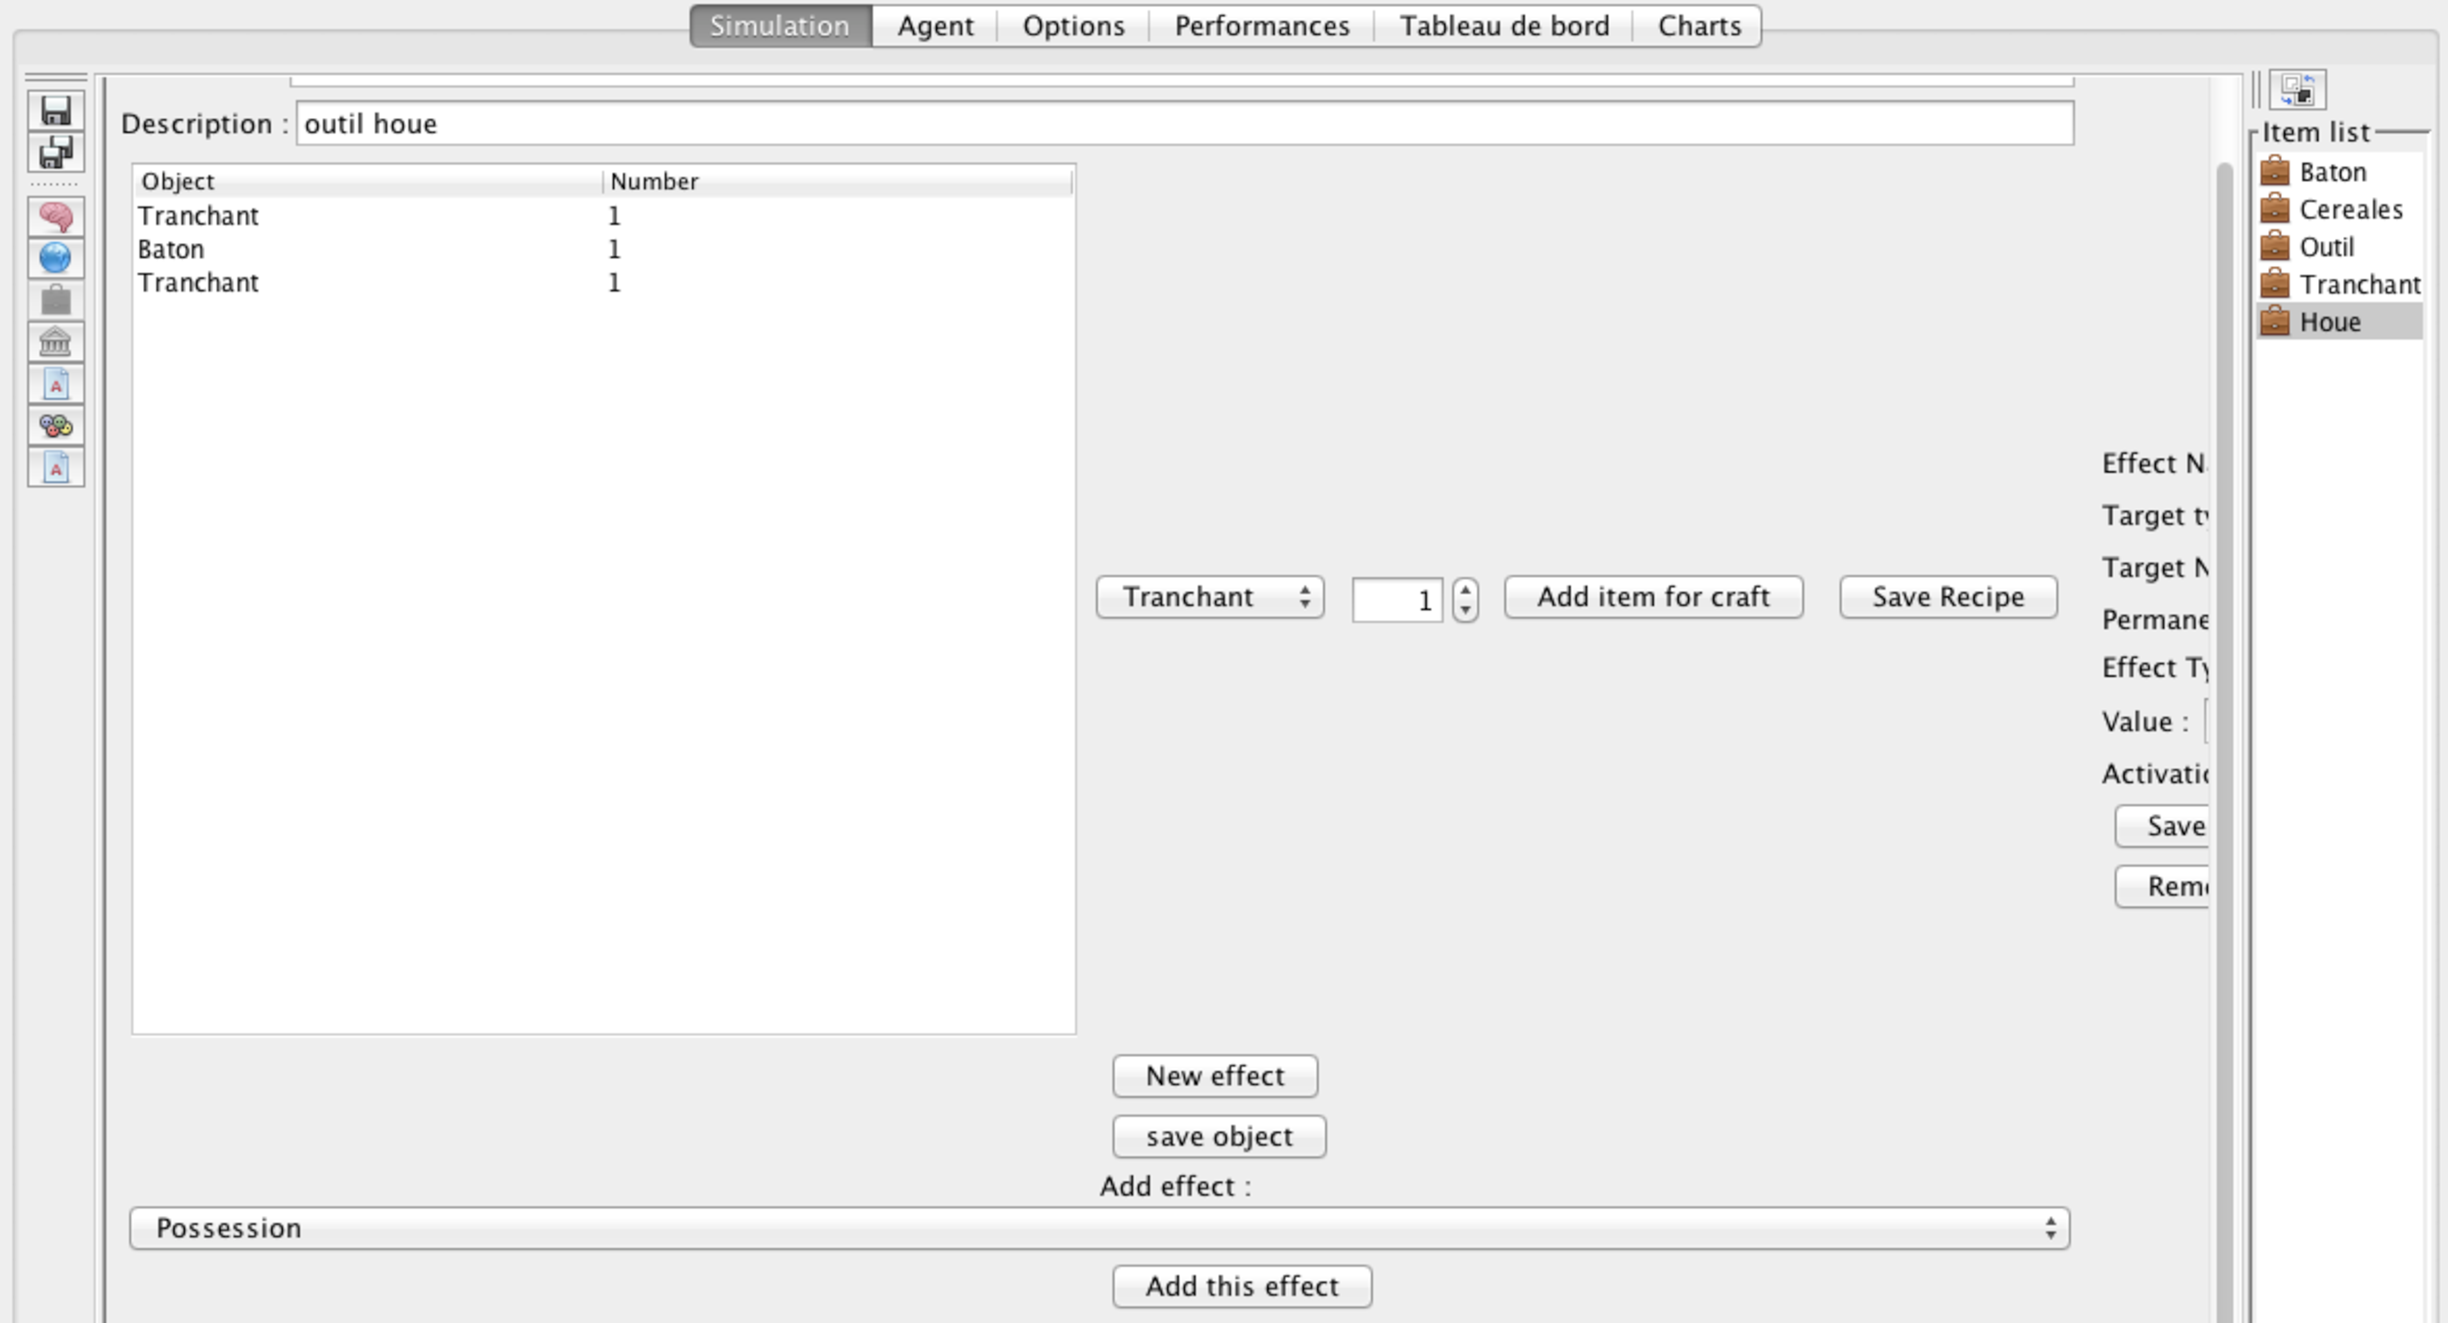
\includegraphics[scale=0.3]{DocumentationSimulation/Objet2.pdf}
	\caption[Ob2]{Objet complexe \\}
	\label{Ob2}
	\end{center}
	\end{figure}
	
En ce qui concerne les effets (cf. Figure \ref{EF2}), tout effet a un nom, une cible qui peut être un attribut (caractéristique de l'agent) ou un cogniton % action. 
Le type de cible étant choisi, on détermine la cible exacte, la durée de l'effet (permanent ou non c'est-à-dire  lié à la durée de vie de l'objet), ce qu'il fait (\textit{set, add, remove}) sur la cible en terme de valuation et en fonction de toute action relative à la création, à l'utilisation et à la destruction de l'objet auquel l'effet est rattaché.

\begin{figure}[!ht]
	\begin{center}
	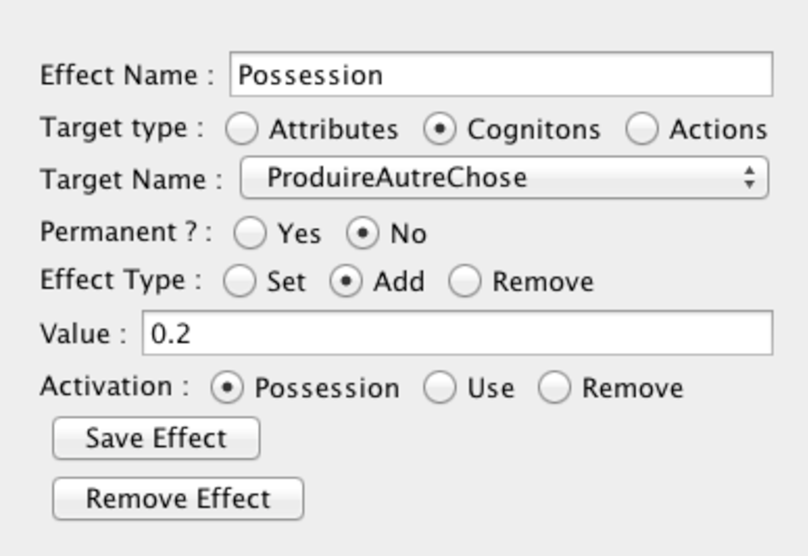
\includegraphics[scale=0.6]{DocumentationSimulation/effet.pdf}
	\caption[EF2]{Effet pour un objet \\}
	\label{EF2}
	\end{center}
	\end{figure}
	
	Exemple, l'objet \textit{Houe} a pour effet \textit{Possession} dont la cible est le cognition \textit{Produireautrechose}, cet effet est transitoire (appliqué tant que l'agent possède la houe), son action sur le cognition est \textit{add} (ajouter) la valeur 0.2 au poids de celui-ci, son activation sera effective chaque fois qu'un agent ajoutera une \textit{Houe} à son inventaire.

\newpage
	
	
\subsection{Les aménagements ou infrastructures}	
		Dans la fenêtre \textit{Wiewertabs}, clicquer sur l'icône \textit{Edit amenagement}, sur la droite on dispose de la liste des aménagements existants.
Pour créer un nouvel aménagement, cliquer sur l'icône \textit{create new amenagement}, donner son nom (par exemple Champ) et sauvegarder.

\begin{figure}[!h]
	\begin{center}
	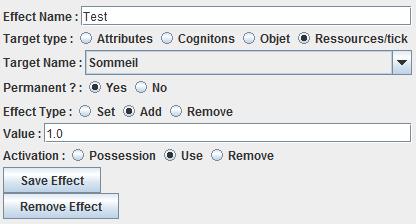
\includegraphics[scale=0.6]{DocumentationSimulation/images/effetsA.png}
	\caption[EFA]{Effet pour un aménagement \\}
	\label{EFA}
	\end{center}
	\end{figure}

 Tout comme pour les objets,  il est possible de saisir une recette pour la conception d'aménagements complexes, le processus étant identique à celui présenté dans la section sur les objets.
 De même, les aménagements peuvent avoir des effets ceux ci étant un peu différents de ceux présentés pour les objets (cf. Figure \ref{EFA})
 
 En effet,  les aménagements  ont la possibilité d'avoir pour cible (en sus des attributs ou caractéristiques d'agent et des cognitions)  des objets ou des ressources, et dans ce cas, l'effet ajoutera, modifiera ou bien supprimera l'objet sélectionné de l'inventaire, ou bien, modifiera, ajoutera, modifiera ou supprimera la ressource ciblée présente sur le patch où se situe l'aménagement.
	
\section{Phase de modélisation}

\subsection{Le schéma cognitif}

\begin{figure}[!ht]
	\begin{center}
	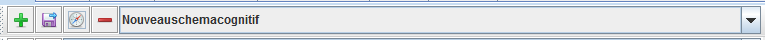
\includegraphics[scale=0.6]{DocumentationSimulation/images/ToolbarSchemaCognitif.png}
	\caption[Interface]{Barre d'outils des schémas cognitifs\\}
	\label{Interface d'édition de cogniton}
	\end{center}
	\end{figure}

Le détail de ces icônes :

\begin{enumerate}
\item Signe plus vert : créer un nouveau schéma cognitif , permet de choisir un nom et propose de copier un schéma cognitif.
\item Disquette : importer un schéma cognitif à partir d'un dossier
\item Boussole : éditer les options du schéma cognitif.
\item Signe moins : supprimer le schéma cognitif sélectionné .
\item Sélecteur : permet de sélectionner le schéma cognitif à éditer.
\end{enumerate}


\subsection{Le canevas : cogniton, plan, action}

	La création d'un nouveau cogniton se fait en cliquant sur l'icône 
\includegraphics{DocumentationSimulation/images/newcogni.png}. 
	
	Un nouveau cogniton est alors créé sous la forme d'une ellipse portant le nom "Nouveau cogniton". 
	
\begin{figure}[!ht]
	\begin{center}
	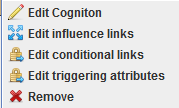
\includegraphics[scale=0.6]{DocumentationSimulation/images/interface.png}
	\caption[Interface]{Interface d'édition de cogniton\\}
	\label{Interface d'édition de cogniton}
	\end{center}
	\end{figure}

Un clic droit sur ce dernier permet d'ouvrir l'interface d'édition (cf. Figure \ref{Interface d'édition de cogniton}). 

Le premier lien permet de donner le nom du cogniton, son type (\textit{ Belief} s'il s'agit d'une croyance de l'agent, même si il s'agit d'une croyance populaire, \textit{Percept} s'il s'agit d'une perception de l'agent, \textit{Skill} s'il s'agit d'une compétence ou d'un savoir-faire, \textit{Trait} s'il s'agit d'une caractéristique psychologique de l'agent et \textit{Culturon} s'il s'agit d'un cogniton partagé par un groupe), et ses pourcentages de chances d'apparition au lancement de la simulation.

Vient ensuite l'édition des \textit{liens d'influence}, à savoir, spécifier quels plans vont être influencés par ce cogniton et dans quelle mesure vont ils l'être. Pour cela, l'on doit sélectionner le plan à influencer ainsi décider le poids de cette influence sur le plan en question. Une fois toutes les influences définies cliquer sur le bouton \textit{OK} pour les enregistrer dans la simulation.

Dans le même menu se trouve l'édition des\textit{ liens conditionnels}. Ces liens spécifient les actions pour lesquelles ce cogniton doit exister obligatoirement dans l'esprit de l'agent pour qu'elle s'exécute. Pour les spécifier il suffit de sélectionner un à un les plans à lier avec l'existence de ce cogniton dans la liste déroulante, puis, cliquer sur le bouton \textit{OK} pour terminer.

Enfin cette interface permet la création de \textit{triggers}. Ces \textit{triggers} permettent de réguler l'apparition d'un cogniton dans l'esprit d'un agent en fonction de la valeur des caractéristiques de ce dernier. Comme un \textit{trigger} est un déclencheur du type \textit{si condition alors}, la création d'un \textit{trigger} se fait en définissant la condition de déclenchement, c'est-à-dire, en sélectionnant la caractéristique de l'agent à comparer, la fonction de comparaison à utiliser, et enfin, la valeur de comparaison. Le cogniton ne se déclenchera, ainsi, dans l'esprit de l'agent, que si cette condition est respectée. 
Il est possible de définir plusieurs conditions au sein d'un même 
 \textit{trigger} . Une fois ces conditions définies, cliquer sur le bouton \textit{OK} pour finir la création du trigger.
 

	

\newpage
\part{Exemple de simulation }
\Large{\emph{La simulation AgriculteurMaisonBois2}}
 	\section{Le modèle}
		\subsection{Peuplement et environnement}
Dans cette simulation, un seul peuplement Civ1 avec une centaine d'agents.

Ceux-ci, ont initialement tous les mêmes caractéristiques : sommeil (50) et vie (20).

La simulation aura lieu dans un environnement constitués de \textit{patches} de deux types de  terrains : forêt et prairie de \textit{passability} 25 et 35.

Après chargement de l'environnement Test.metaciv, on dispose de l'environnement et de la localisation de départ de Civ1 (cf. Figure \ref{loca})
\begin{figure}[!ht]
\begin{center}
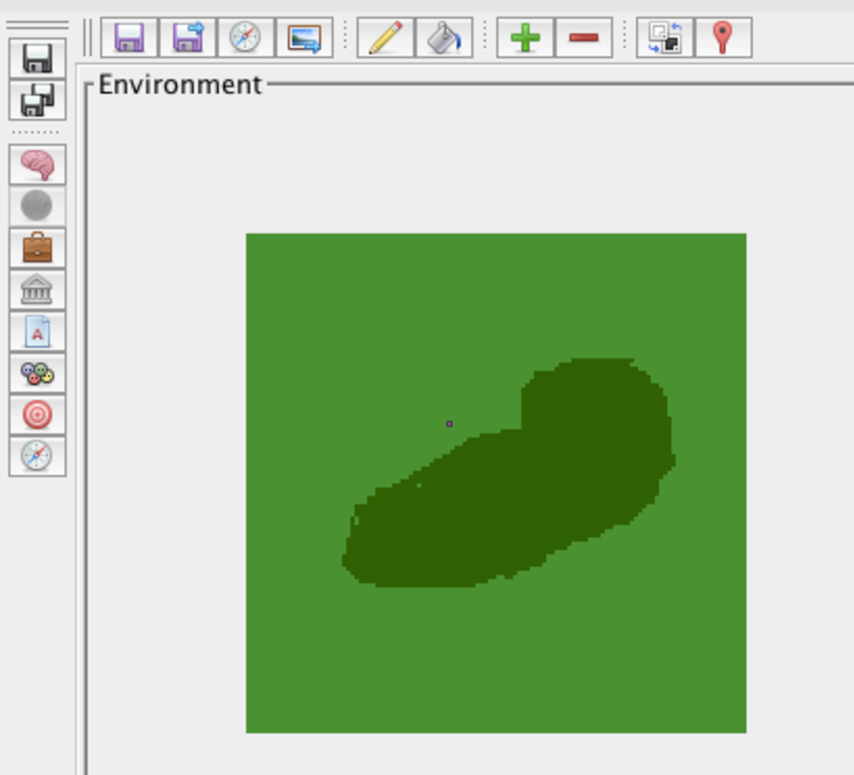
\includegraphics[scale=0.5]{DocumentationSimulation/locas1.pdf}
\caption[loca]{Environnement \\}
\label{loca}
\end{center}
\end{figure} 

L'inventaire des agents pourrait potentiellement comporter les objets Baton, Céréale, Outil.

Céréale a l'effet possession qui ajoutera 0.2 au poids du cogniton \textit{Produireautrechose  }à chaque fois qu'un agent ajoutera un objet céréale à son inventaire.

En ce qui concerne les aménagements \textit{(facility)}, on trouve Champ et Maison.
Champ a un effet permanent \textit{Renforcer agriculture } qui ajoute  0.05 au poids du cogniton \textit{Agriculteur} à chaque fois qu'il utilise le champ.

Maison a un effet permanent \textit{Dormir} qui ajoute 40.0 à l'attribut \textit{Sommeil} de l'agent à chaque fois qu'il utilise cet aménagement.

\subsection{Cogniton, Plan, Actions}



\begin{figure}[!ht]
\begin{center}
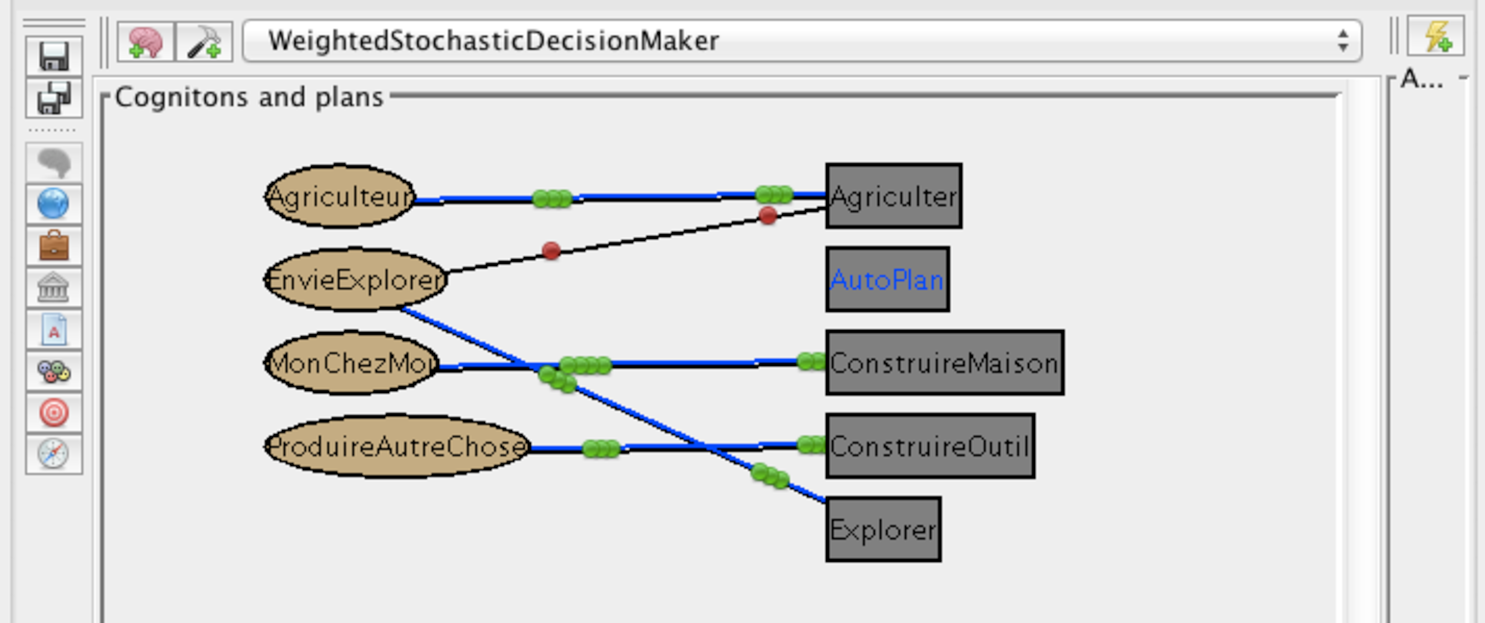
\includegraphics[scale=0.5]{DocumentationSimulation/CogPl.pdf}
\caption[CP]{Environnement \\}
\label{CP}
\end{center}
\end{figure} 

La figure \ref{CP} présente la \textit{cognition} : l'ensemble des cognitons (Agriculteur, EnvieExplorer, MonChezMoi, ProduireAutreChose) et plans (Autoplan et Agriculter, ConstruireMaison, ConstruireOutil, Explorer) ainsi que les liens conditionnels (bleu) et d'influence (noir).

Les billes vertes correspondent à une influence positive, les rouges à une influence négative et leur quantité dénonce le poids.

Par exemple, Agriculter est lié conditionnellement au cogniton Agriculteur (qui influence aussi positivement ce plan) ; par contre  le cogniton EnvieExplorer influence négativement ce même plan.

Un clic droit sur chaque cogniton donne le détail sur celui-ci (nom, type et pourcentage d'agent qui auront ce cogniton à leur création) et sur les liens le concernant.

\textit{Remarque : le dosage du pourcentage est important dans le modèle et pour la simulation}

Pour accéder à la description des actions d'un plan (clic gauche), si les actions L double cliquer sur elles jusqu'à déploiement complet des actions du plan.


\begin{flushleft}
\textbf{Autoplan}
\end{flushleft}

	2 actions A\_ChangeAttribute (portant sur sommeil et vie)
	
	
\begin{flushleft}
\textbf{Plan ConstruireMaison}
\end{flushleft}

L'arbre des actions déployé est représenté sur la figure \ref{PL}.
\begin{figure}[!ht]
\begin{center}
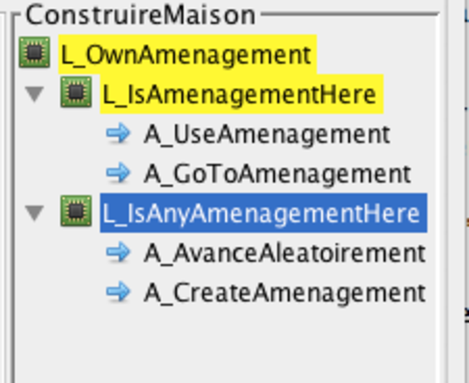
\includegraphics[scale=0.5]{DocumentationSimulation/planex.pdf}
\caption[PL]{Arbre des actions du plan ConstruireMaison \\}
\label{PL}
\end{center}
\end{figure} 

\begin{algorithm}
\caption{Plan ConstruireMaison}
\label{Com}

\Begin{
   
     
    \If{j'ai une maison (n'importe où) }
   {
        \If{j'ai une maison sur le patch où je suis}
  		 	{   
  		 		\texttt{action interne 1 niveau 1}
  		 		
       		 	j'utilise cette maison (et par suite je gagne 40 de sommeil)
   			}	   
        	\Else
        	{
        		\texttt{action interne 2 niveau 1  }
        		
        		je me déplace vers le patch de ma maison la plus proche
        	}
   }    

    \Else
    {
       		\If{sur le patch où je suis, existe un quelconque aménagement }
  		 	{
  		 		\texttt{action interne 1 niveau 2 }
  		 		
       		 	 j'avance aléatoirement d'un pas (le patch étant occupé)
   			}	   
        	\Else
        	{
        		\texttt{action interne 2 niveau 2} 
        		
        		je crée une maison sur le patch
        	}
   }    
 }
\end{algorithm}

Cette action permet à l'agent de construire l'aménagement souhaité si celui n'en possède pas déjà un et qu'il n'y a pas d'aménagements sur le patch sur lequel il se trouve. Si le patch est occupé il ira en chercher un libre plus loin. Si l'agent possède déjà cet aménagement il ira l'utiliser.

Les autres actions de constructions sont construites de la même manière.

		\clearpage
	\section{Observation de la simulation}
		Une fois la simulation lancée. Le tick 1 crée la position de départ du peuplement. Le tick 2 crée les agents. Il est possible, à partir du tick 3, de sélectionner un agent (avec un clic gauche) et de l'observer (au moyen d'un clic droit suivi de la sélection du choix \textit{Observe one agent}). Cette fenêtre d'observation se met à jour automatiquement à chaque tick de la simulation. Elle permet ainsi d'observer facilement l'évolution d'un ou plusieurs agents au cours de la simulation.

\subsection{La fenêtre d'observation d'un agent}

Le premier onglet, l'onglet \textit{Mind}, qui s'ouvre automatiquement, représente les cognitons et les plans présents dans l'esprit de l'agent. Il permet d'observer rapidement la répartition des cognitons et des plans dans l'esprit de l'agent (cf. Figure \ref{observe}).

\begin{figure}[!ht]
\begin{center}
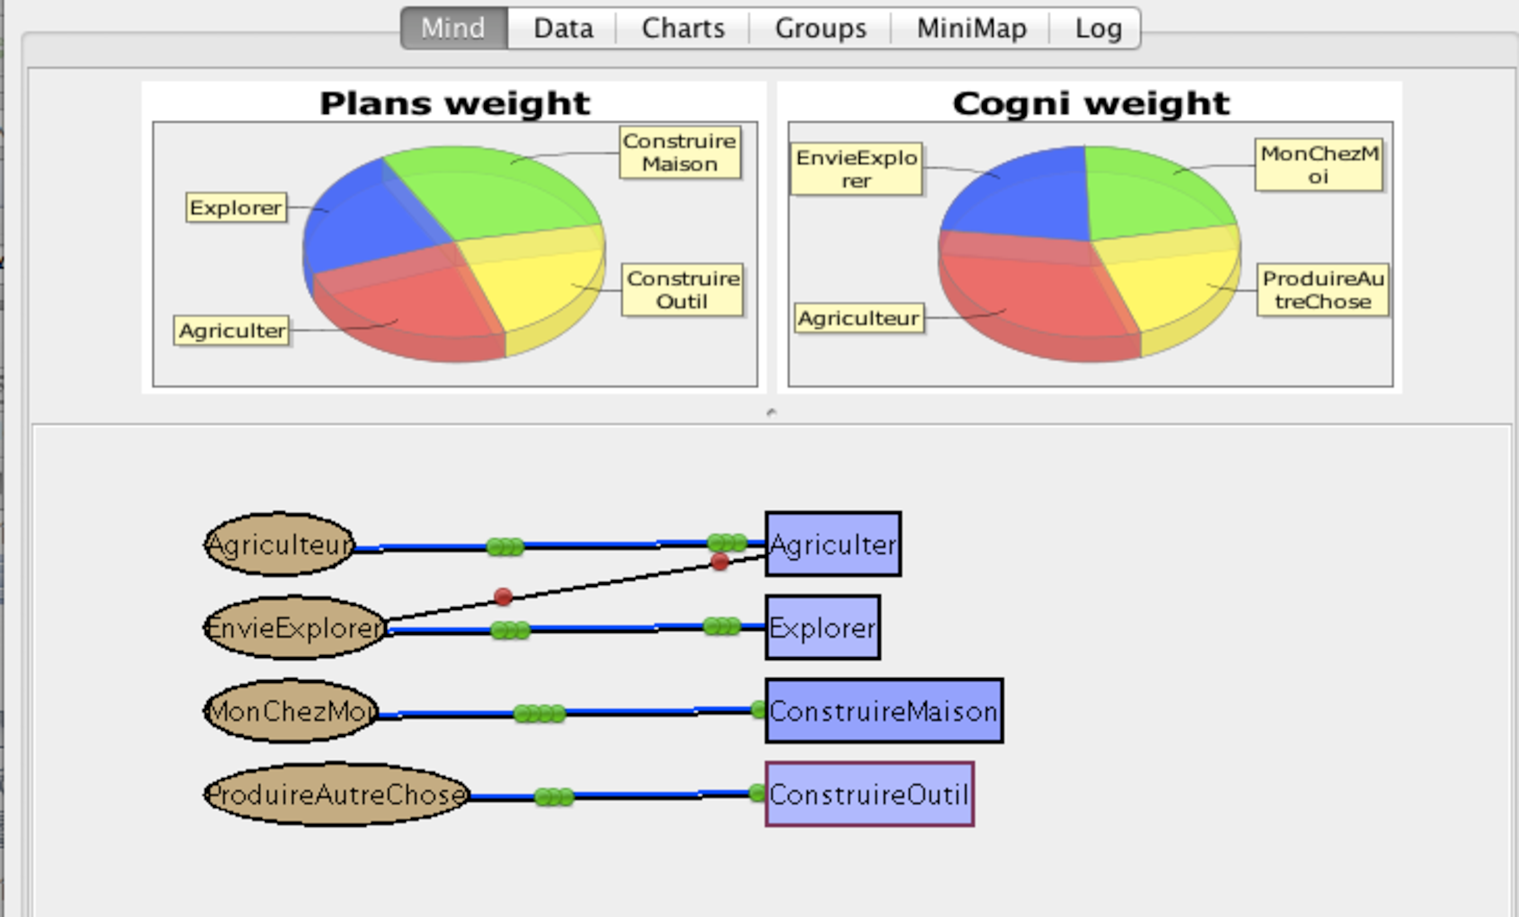
\includegraphics[scale=0.5]{DocumentationSimulation/observe.pdf}
\caption[observe]{Fenêtre d'observation de la constitution de l'esprit de l'agent \\}
\label{observe}
\end{center}
\end{figure} 

Cela permet ainsi, au moyen du graphique \textit{Cogni weight}, de voir que, au tick auquel a été prise cette impression d'écran, l'agent observé possédait les quatre cognitons EnvieExplorer, Agriculteur, MonChezMoi et ProduireAutreChose avec un poids un peu plus important pour le cogniton Agriculteur. De même on peut aussi voir que cet agent est susceptible, à ce tick, d'effectuer les plans Explorer,Construire Outil, Construire Maison et Agriculter avec un peu plus de chances pour le plan Construire Maison et Agriculter. 


L'onglet \textit{Data }présente une vision globale des données concernant l'agent, à savoir, le poids de ses cognitons, le poids des plans qu'il est susceptible d'effectuer, la valeur de chacun de ses attributs, son inventaire, le plan qu'il effectue au cours de ce tick, ainsi que le type de patch sur lequel il se trouve (cf. Figure \ref{observe2}) ou même les groupes auxquels il appartient.

\begin{figure}[!ht]
\begin{center}
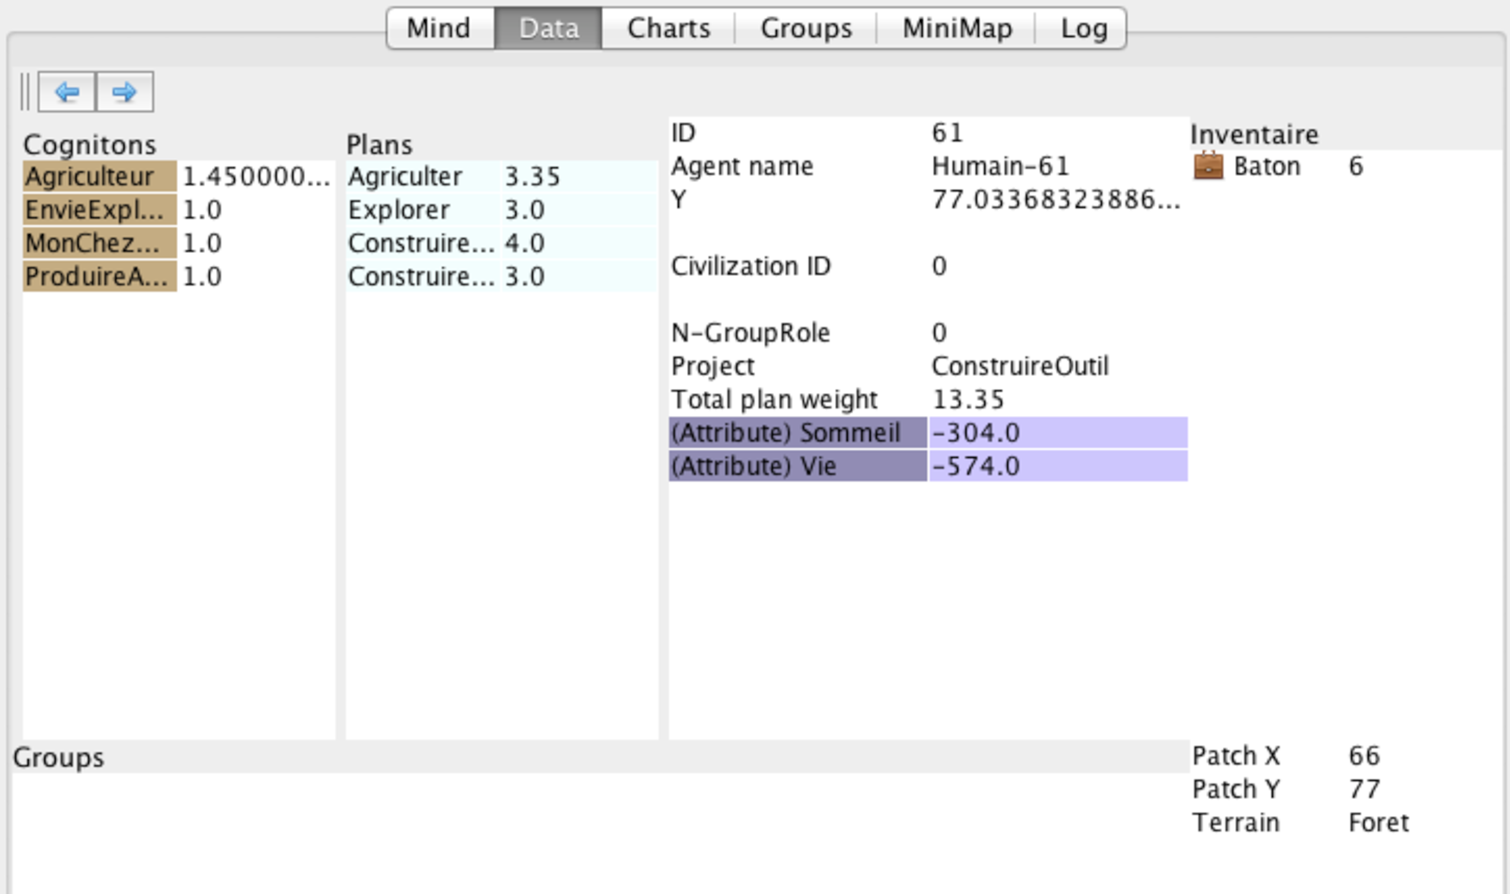
\includegraphics[scale=0.5]{DocumentationSimulation/observe2.pdf}
\caption[observe]{Fenêtre d'observation de l'agent \\}
\label{observe2}
\end{center}
\end{figure} 

Dans le cas de cette simulation et à ce tick précis, on peut voir que l'agent observé possède le cogniton Agriculteur, lequel a un poids de 1.45, les autres cognitons présents dans l'esprit de l'agent ont un poids de 1.0 ce qui confirme l'information donnée par le premier onglet, il en est de même concernant les plans. On peut aussi constater que l'agent possède 6 objets Bâton dans son inventaire et que son plan actuel est Construire\_Outil. Il est donc prévisible qu'au prochain tick, l'agent crée un outil à partir de ces bâtons. De plus on observe que l'agent possède ces deux attributs Vie et Sommeil largement en négatif, ce qui est normal, car rien n'a été  prévu, dans cette simulation, lors de la création de la cognition de l'agent, pour pousser ce dernier à consommer de la nourriture ou à aller se reposer si ses attributs atteignent un seuil critique. Il aurait été possible de le faire en définissant un \textit{trigger } portant sur l'attribut voulu et déclenchant l'apparition d'un cogniton influençant très positivement un plan consistant à augmenter la valeur de cet attribut. Enfin cet onglet nous permet de constater que l'agent n'appartient à aucun groupe et qu'il se situe sur un patch de type Forêt.

L'onglet \textit{Charts} contient deux graphiques représentant, pour le premier, la répartition des attributs de l'agent, et le second, un aperçu rapide de la valeur de chaque plan de l'agent. Passer la souris sur chaque composante des graphiques permet d'obtenir plus d'informations (cf. Figure \ref{observe3}).

\begin{figure}[!ht]
\begin{center}
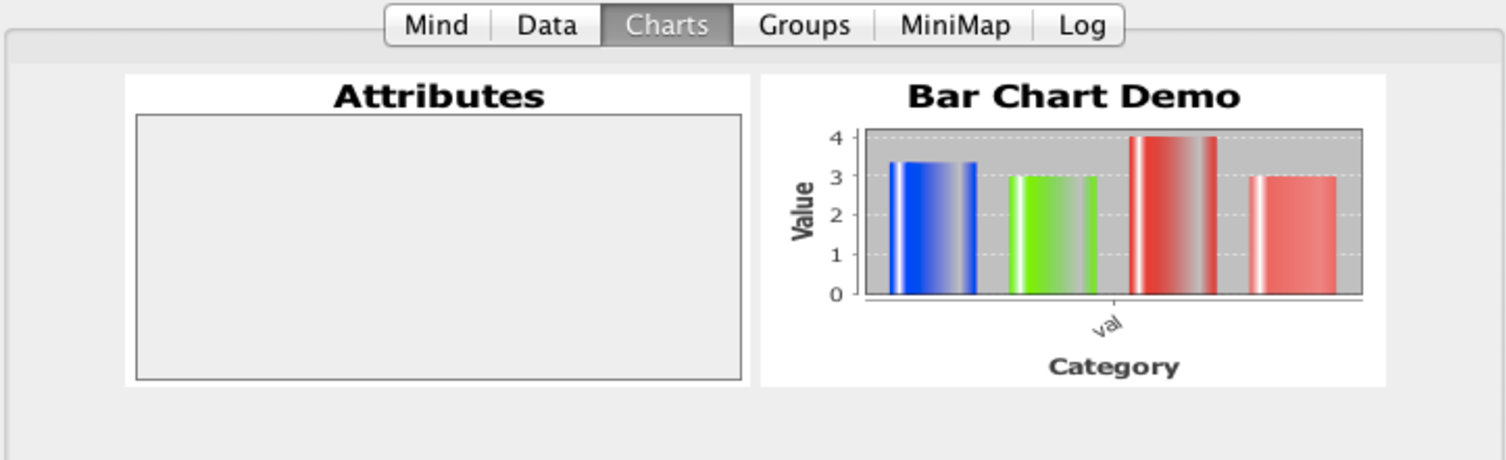
\includegraphics[scale=0.5]{DocumentationSimulation/observe3.pdf}
\caption[observe]{Fenêtre d'observation des attributs et plans de l'agent \\}
\label{observe3}
\end{center}
\end{figure} 

Cet onglet permet ainsi de confirmer que les valeurs des attributs de l'agent sont négatives car elles n'apparaissent pas dans le graphique et nous montre le poids de chaque plan susceptible d'être effectué par l'agent sous forme d'un diagramme. Pour savoir quel plan est représenté par quelle couleur il suffit de passer la souris au-dessus de celui-ci.



L'onglet \textit{Groups} permet d'avoir une représentation des groupes auxquels appartient l'agent observé, ainsi que son rôle dans ces groupes. L'agent n'appartenant à aucun groupe cet onglet ne nous apprendra rien dans cette simulation, dans d'autres simulations nous pourrions observer les rôles de l'agent observé dans les différents groupes auxquels il appartiendrait.



L'onglet \textit{Minimap} permet d'avoir un zoom sur la position de l'agent sur la carte.



Enfin, l'onglet \textit{Log }permet d'avoir un récapitulatif des plans et des actions effectués par l'agent à chaque tick (cf. Figure \ref{observe4}).

\begin{figure}[!ht]
\begin{center}
\includegraphics[scale=0.5]{DocumentationSimulation/observe4.pdf}
\caption[observe]{Fenêtre récapitulative des actions de l'agent \\}
\label{observe4}
\end{center}
\end{figure} 

Nous pouvons ainsi voir que les derniers agissements de l'agent consistaient à aller se reposer à sa maison puis à aller chercher de quoi fabriquer des outils.


\subsection{La fenêtre d'observation générale}

Il est aussi possible d'observer le comportement général des agents au moyen des onglets \textit{Agents}, \textit{Options}, \textit{Performances}, \textit{Tableau de bord} et \textit{Charts} présentés précedemment.

L'onglet \textit{Agents} correspond à l'onglet \textit{Data} présenté précédemment à ceci prés qu'il est muni de deux flèches avant et arrière permettant de facilement passer de l'observation d'un agent à un autre.

L'onglet \textit{Options} permet de définir les préférences d'affichage de la fenêtre \textit{WorldViewer}. Il est muni de plusieurs options :
\begin{itemize}
\item \textit{Affichage des plans} : permet de n'afficher que les agents effectuant un certain plan à sélectionner dans la liste déroulante. Les agents n'effectuant pas ce plan seront minimisés et ne seront visibles qu'en cas de zoom.
\item \textit{PheroMap} : permet de colorer les patches non plus en fonction de leur type de terrain mais en fonction de la valeur de la ressource sélectionnée pour chaque patch. Plus la ressource est présente sur le patch, plus ce dernier sera coloré en bleu.
\item \textit{ShowSpecificGroupAndRole} : permet de colorer les agents en fonction de leur appartenance à un groupe.
\end{itemize}

L'onglet \textit{Performances} quand à lui affiche les ressources matérielles utilisées par la simulation.

L'onglet \textit{Tableau de bord} permet, en cliquant sur l'icône \textit{Mettre à jour les données} représentée par une double disquette, de visualiser pour chaque cogniton, le pourcentage d'agents présents dans la simulation le possédant. 
% à voir

Enfin l'onglet \textit{Charts} permet de voir l'évolution de la moyenne des poids de chaque plan dans l'esprit des agents composants la simulation, de même pour les attributs.


\end{document}